
\chapter{小型涵道式无人机的系统构成与建模}
系统建模是涵道式无人机的飞行控制和理论分析的底层核心环节。将涵道式无人机看作一个非线性系统，则其无人机的机电系统就是其基础和底层实现，决定着整个非线性系统的上限。本章首先介绍用于实验的涵道式无人机的机电控制系统。接着，为了便于分析，阐述了本文所使用的坐标系并定义了相对应的符号。然后，基于实验对象为刚体的假设，采用牛顿-欧拉法对无人机进行运动学分析。最后，参考现有涵道式无人机的动力学分析理论，对实验对象进行动力学分析，给出涵道式无人机的非线性系统方程。

\section{涵道式无人机的系统构成}
\subsection{机体结构}
涵道式无人机大致结构如图\ref{fig:body}所示。顾名思义，涵道式无人机的核心结构是螺旋桨以及涵道壁。涵道风扇的转轴所在的直线被称为机体轴，该无人机具有C4旋转对称性，即机体绕机体轴旋转90°后，其几何结构与质量分布均与原状态重合。无人机选用直径为7寸的螺旋桨作为内部的涵道风扇。螺旋桨和其外包裹的筒状涵道壁共同构成完整的涵道结构。涵道壁内径略大于螺旋桨直径，用于约束气流，使内部气流保持轴向流动。

为抵抗螺旋桨高速转动产生的反扭距，在螺旋桨的下方装有反扭距襟翼。该襟翼有四片固定的机翼构成，各机翼平行于机体轴，且围绕机体轴成星型排布，如图\ref{fig:body}涵道风扇下方的灰色结构所示。

反扭距襟翼下方装有四个由舵机控制的可旋转的控制舵面，每个控制舵面由两片平行翼面构成，用于产生控制力矩，对整机进行闭环控制。为了增加控制舵面产生的气动力对无人机质心的力臂，无人机的质心需要往上移，因此，电池、电机和电调被设计在无人机的顶部。

机上搭载有两块电路板，分别是飞行控制板和舵机驱动板，各自搭载一块微控制器。舵机控制板位于无人机的底部，而飞行控制板位于电池上方，距离质心较近。飞行控制板上搭载有IMU和气压计等对温度、气压较为敏感的器件，为此专门设计了飞行控制板仓室外壳用于将它们与外界空气隔离。
\begin{figure}
    \centering
    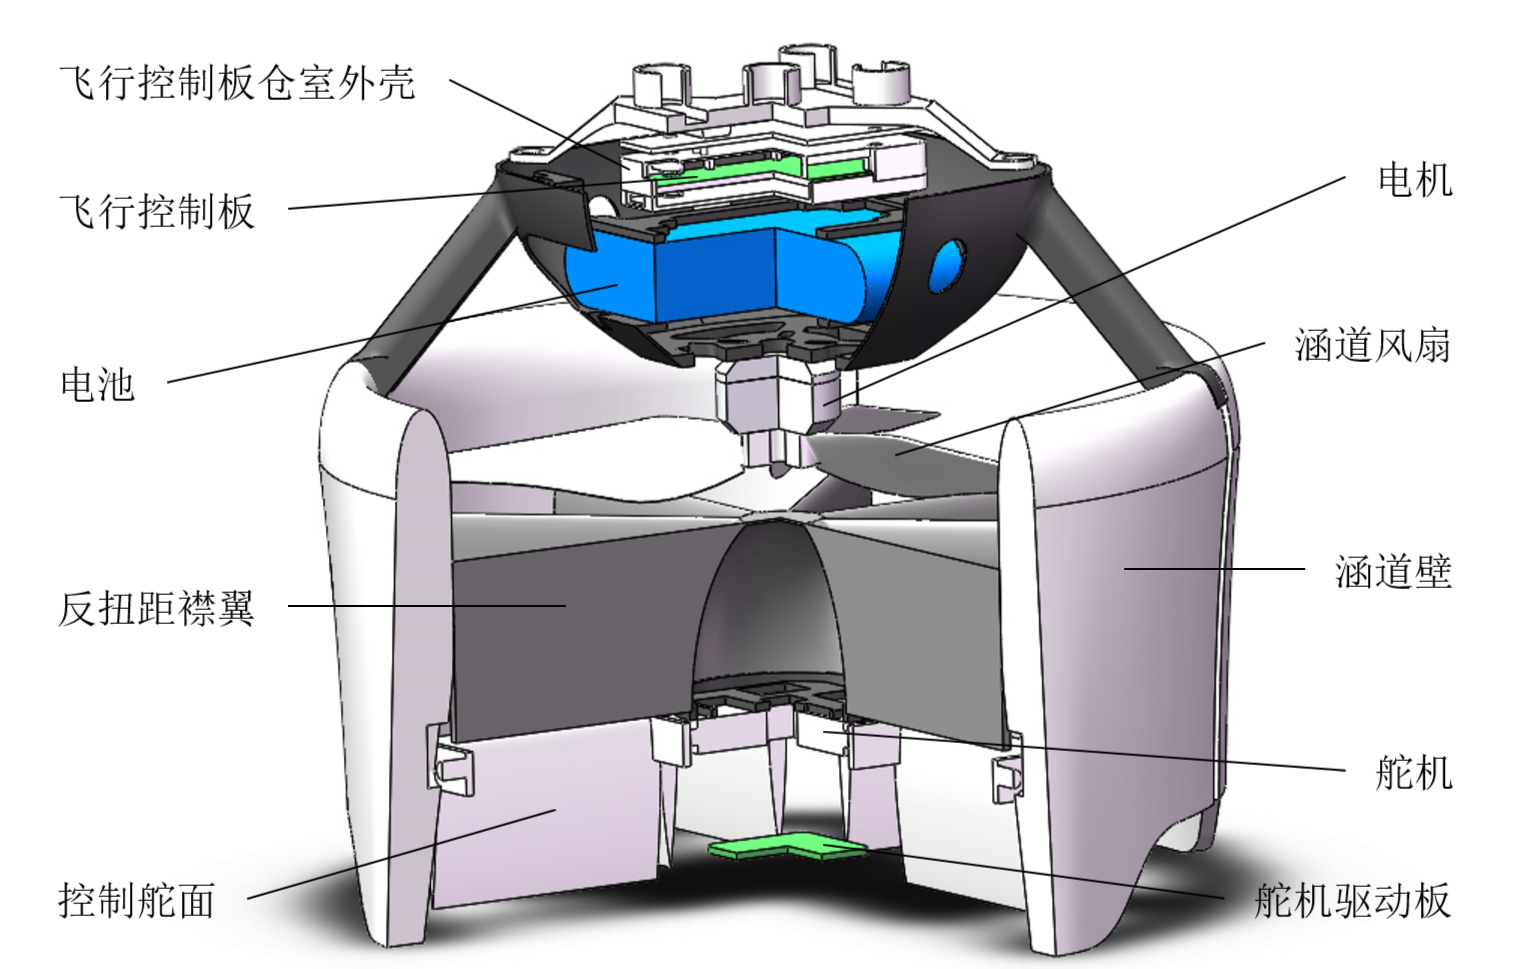
\includegraphics[scale=0.25]{figure/chapter2/ductedfan_parts.png}
    \caption{\label{fig:body}机体结构}
\end{figure}
\subsection{机电控制系统}
机电控制系统是是无人机的“大脑”和“神经中枢”，负责感知自身状态、处理信息并精确控制各个执行机构。其主要包括微控制器，传感器和执行器。接下来将对该无人机附带的机电控制系统的各个模块进行逐一介绍。

\begin{itemize}
    \item \textbf{微控制器}：本文使用的为控制为意法半导体公司的STM32系列的STM32F767芯片，基于ARM架构的Cortex-M7内核设计。最高主频可达 216MHz。集成单精度浮点运算单元FPU和DSP指令集，能够轻松胜任飞行控制环节中的自身状态感知算法和闭环控制算法。此外，集成了PWM、IIC、SPI、UART等常用通信接口，能够与其它硬件模块实现低时延高可靠的通信。同时，片内集成2MB的的Flash存储器与 512KB 的SRAM存储器，能够提供充足空间来执行内存占用较大的高阶卡尔曼滤波等算法。
    \item \textbf{惯性测量单元}：惯性测量单元（Inertial Measurement Unit，IMU）能够高频率地采集无人机的角速度和加速度，为飞控计算机提供解算飞行状态所需的原始数据，是无人机的“小脑”。本文使用的惯性测量单元是InvenSense公司的ICM-20602。该芯片量程范围大，支持±2000dps陀螺量程、±16g加速度量程。且测量噪声小，速率噪声典型值为0.004 °/s/√Hz，加速度计噪声典型值为 100 µg/√Hz，该芯片最高采样频率为1kHz。配合上卡尔曼滤波算法能够实现高精度的位姿估计。
    \item \textbf{磁力计}：磁力计用于感知地磁北的方向，在小范围运动的情况下，该方向可以认为与地球北极的方向成一个固定的夹角。本文使用的磁力计是iSentek的IST8310三轴霍尔效应磁传感器。该传感器的测量范围大，支持三轴±1600µT磁感应强度，该量程足以测量地磁场的方向和大小。最高采样频率为200Hz。磁力计的数据能够保证位姿估计时，航向角的估计不会发散。
    \item \textbf{激光测距模块}：激光测距模块被安装在飞机的底部，是无人机领域用于感知离地高度的常用传感器。本文使用的激光测距模块是意法半导体公司的VL53l1X激光测距传感器。测量精度为±5\%，采样频率为50Hz。读取测量数据能够感知离地高度进而能够对地面效应带来的扰动做抗扰控制。
    \item \textbf{电池}：本文使用的电池是容量为1680mAh的4S1P的航模电池，电池的输出电压为16.8V，最大持续输出电流为20A。
    \item \textbf{电机电调系统}：电机电调系统用于带动主螺旋桨的转动。本文使用的电机是翼飞的2806.5无刷直流电机，其KV值为1300KV，定子直径28mm，高度6.5mm。使用的电调的通信方式为PWM通信，控制频率为200Hz。其额定电压为16V，额定电流为30A。
    \item \textbf{无刷电机测速模块}：该测速模块的本质是利用电机绕组在换相过程中产生的反电动势作为转子位置和速度的信息载体。通过检测两相电压，并辅以特定的开关时序，可以提取出反电动势的过零点，最终通过测量这些特征点的时间间隔来实现对电机转速的精确计算，模块通过PWM脉宽将转速信息输出给MCU。
    \item \textbf{舵机}：舵机用于控制螺旋桨下方的控制舵面的转动，是无人机实现姿态闭环控制的关键。本文使用的舵机是银燕的ES9251舵机，该舵机为塑料齿轮舵机，单个舵机重量仅为2.8g，最大输出力矩为0.02646N·m。舵机的通信方式为PWM通信，最高控制频率为50Hz。
    \begin{figure}[htbp]
        \centering
        \begin{minipage}[b]{0.45\textwidth}
            \centering
            
\includegraphics[height=0.14\textheight]{figure/chapter1/STM32.png}
            \caption{微控制器}
        \end{minipage}
        \hfill  % 产生弹性水平间距
        \begin{minipage}[b]{0.45\textwidth}
            \centering
            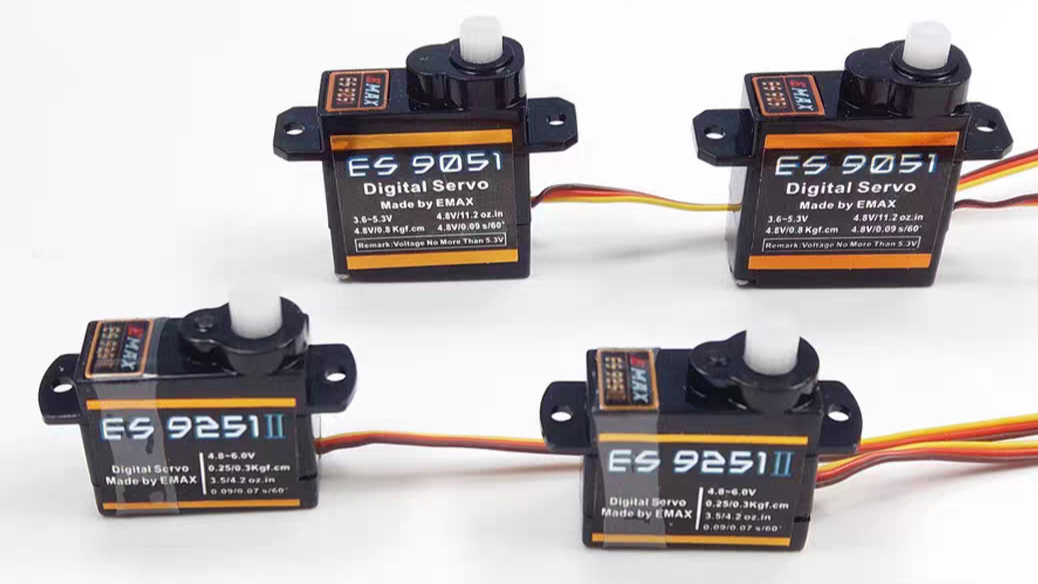
\includegraphics[height=0.14\textheight]{figure/chapter1/servo.png}
            \caption{舵机}
        \end{minipage}
    
        \vspace{0.5cm}

        \centering
        \begin{minipage}[b]{0.45\textwidth}
            \centering
            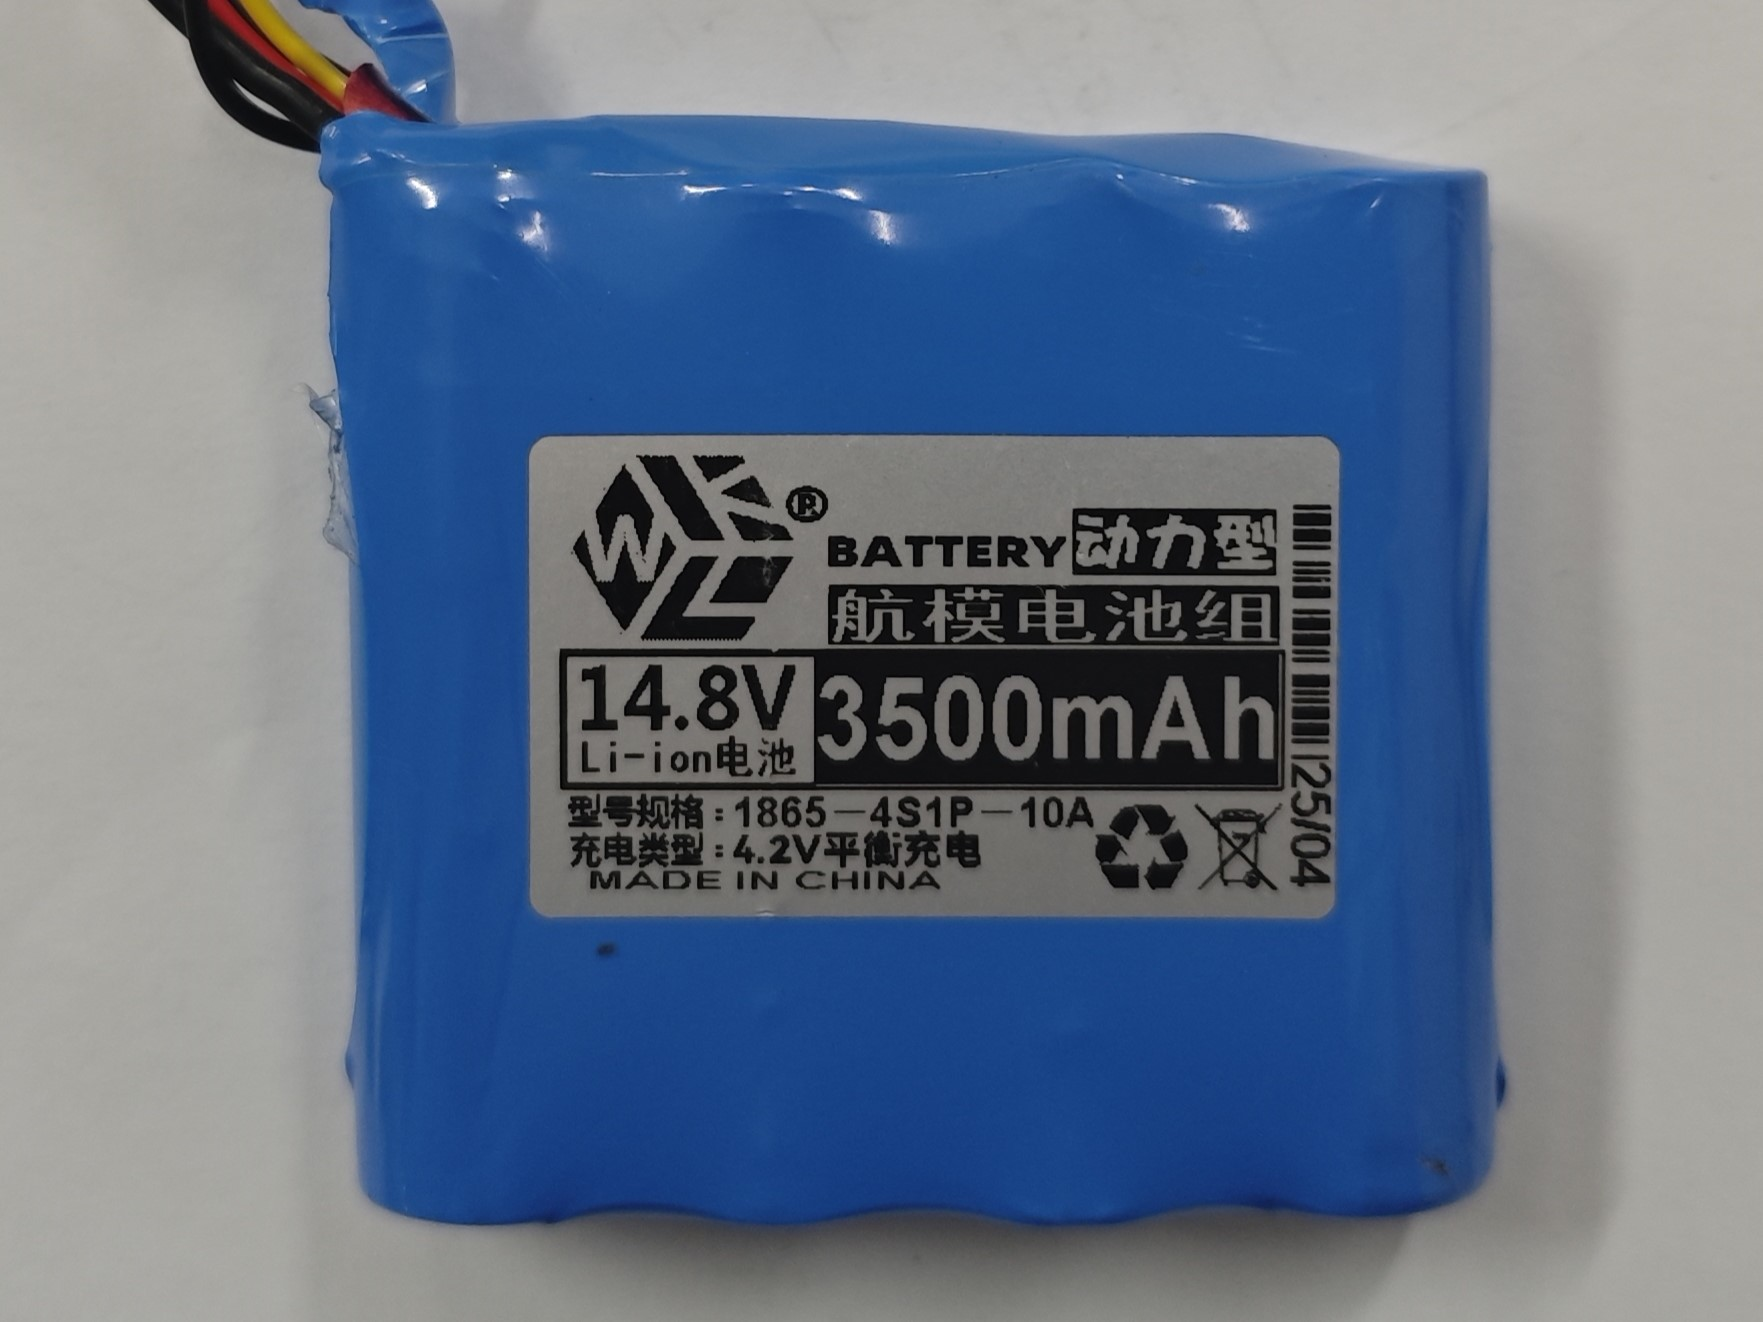
\includegraphics[height=0.14\textheight]{figure/chapter1/battery.jpg}
            \caption{电池}
        \end{minipage}
        \hfill  % 产生弹性水平间距
        \begin{minipage}[b]{0.45\textwidth}
            \centering
            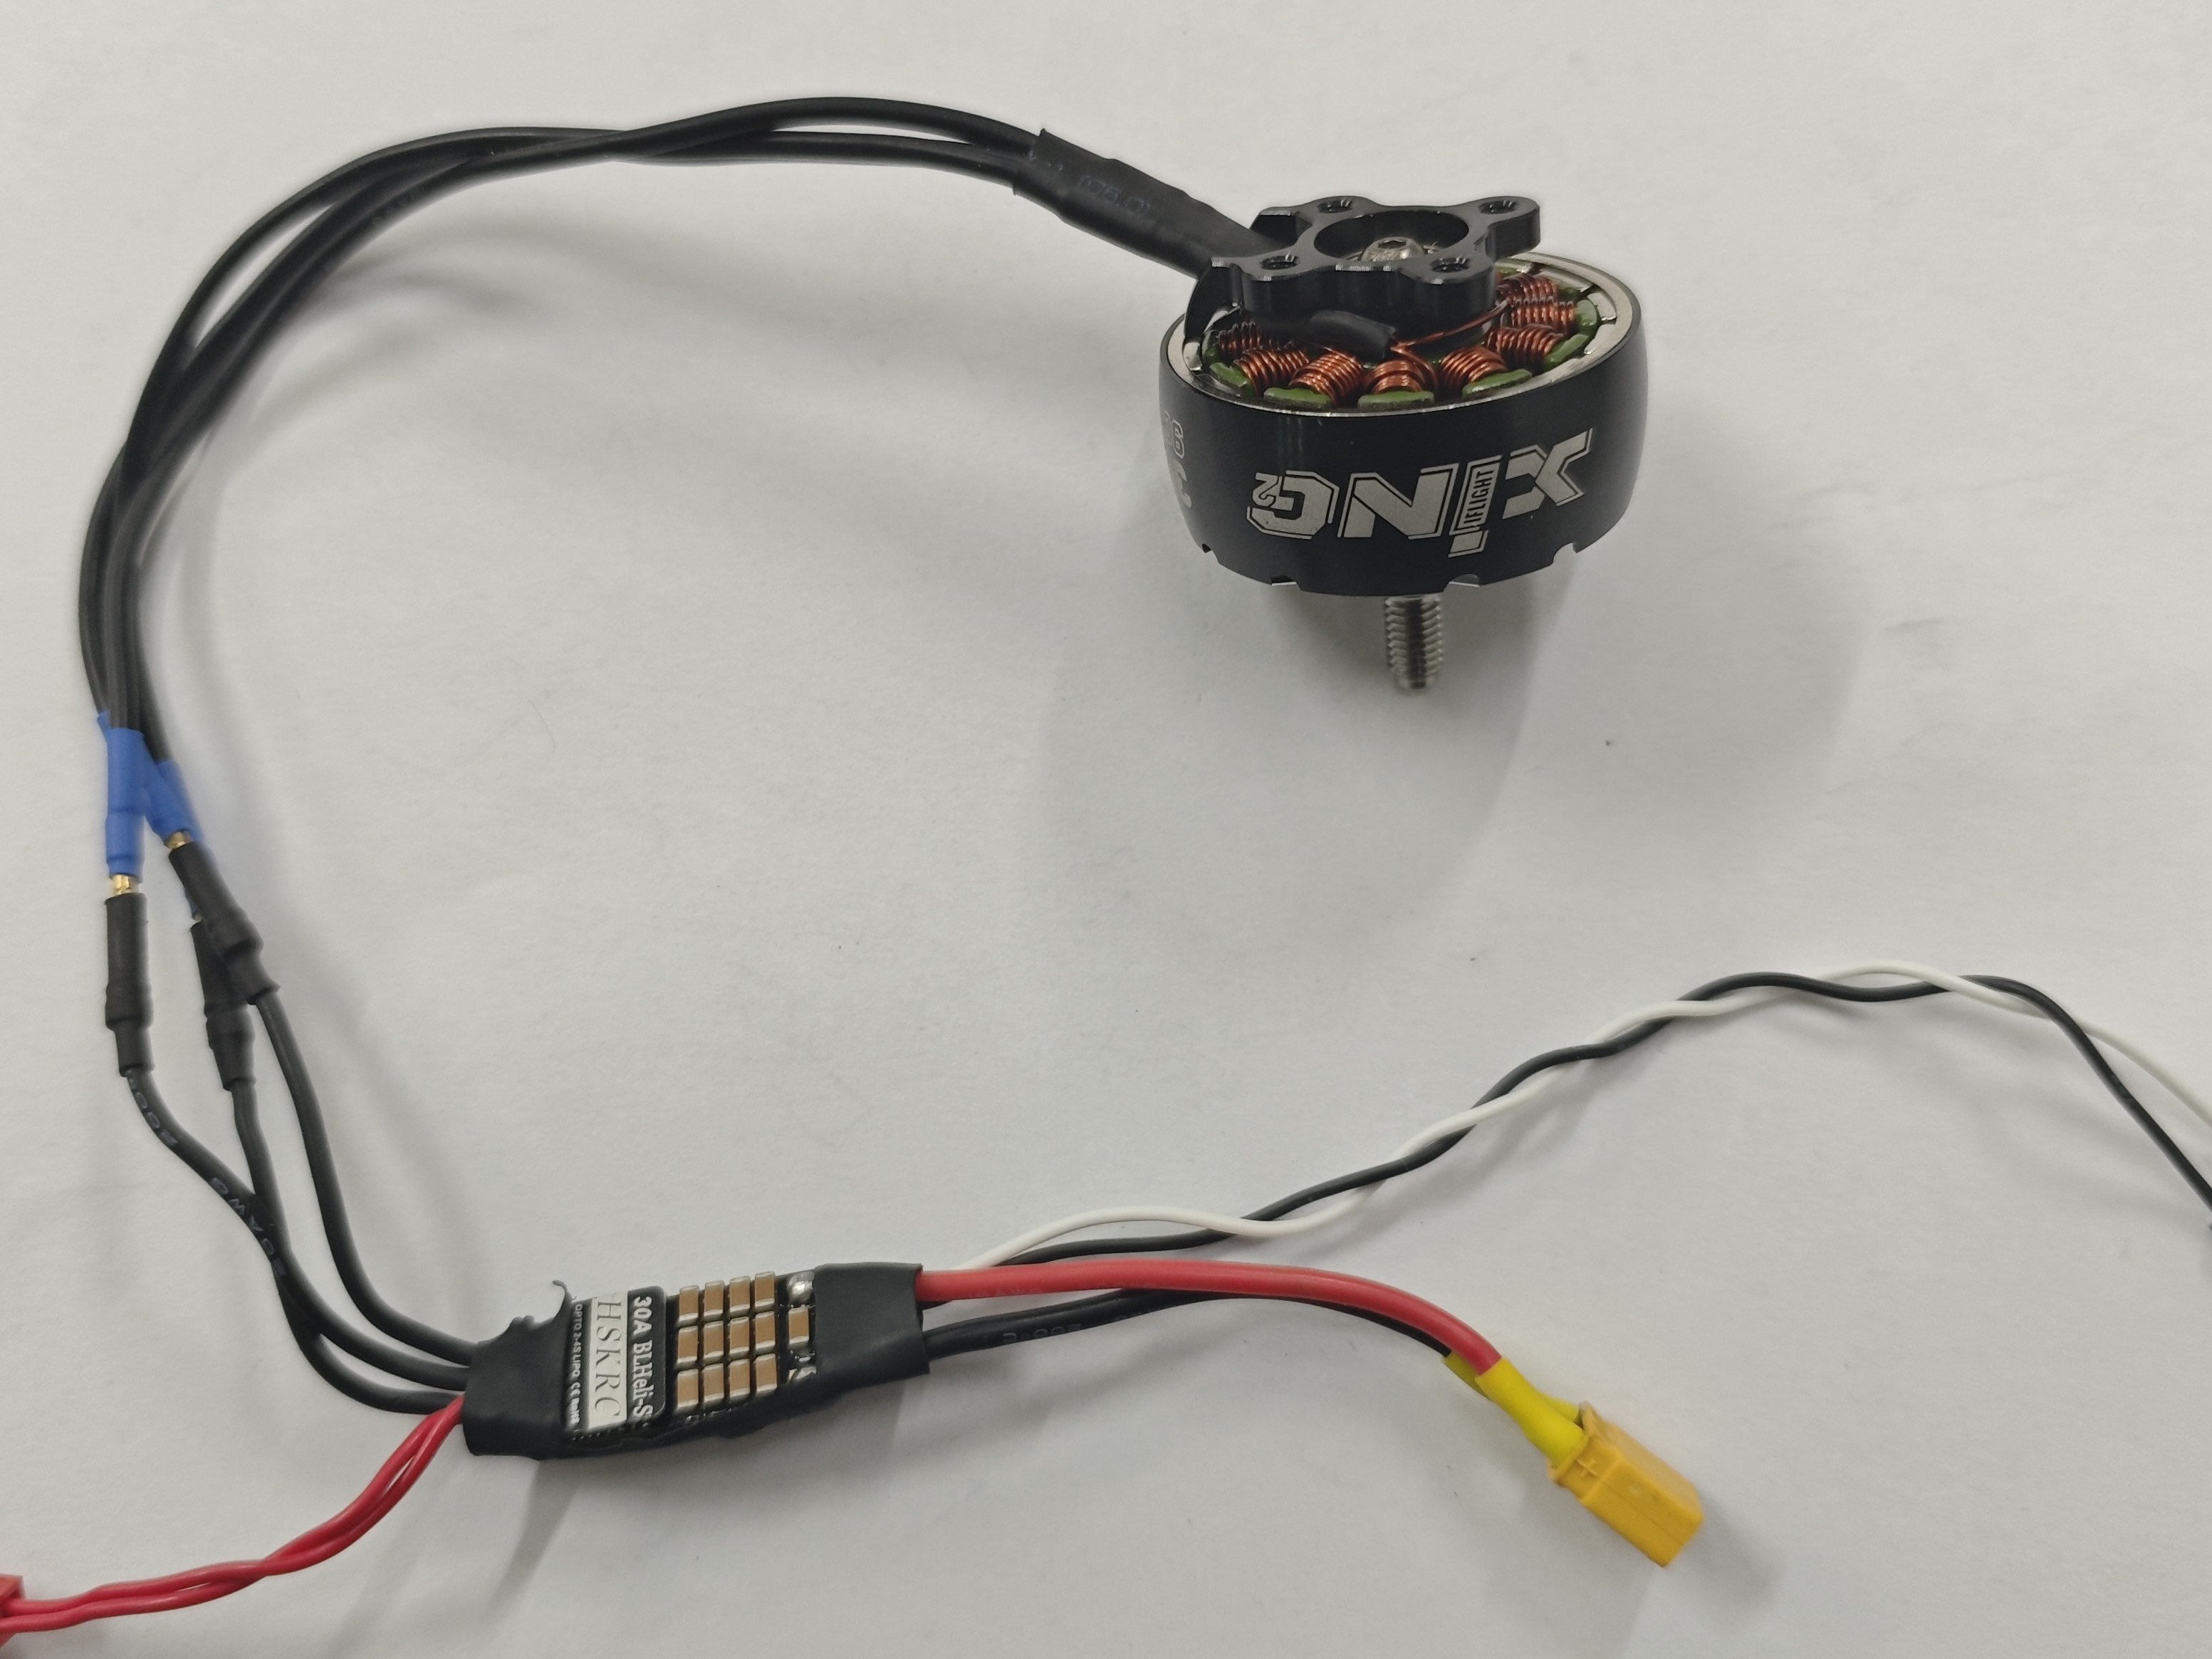
\includegraphics[height=0.14\textheight]{figure/chapter1/motor.jpg}
            \caption{电机电调系统}
        \end{minipage}
    \end{figure}
    
    \item \textbf{电路板}：为了将整个电子系统的各个模块连接起来，独立设计了两块电路板，分别是飞行控制板和舵机驱动板。这两块电路板上各搭载了一块微控制器芯片。电路板将其中搭载的芯片和电子模块通过印制电路连接，并将微传感器的各个物理通信口，通过线对板针座引出。飞行控制板用于执行复杂的位姿估计算法，闭环控制算法，而舵机控制板主要执行指令控制舵机以及获取传感器输出。为了能够测出无人机质心的角速度和加速度，IMU被设计放置在更靠近质心的飞行控制板。而为了使磁力计尽量少地受到无刷电机的磁场干扰，它被设计放置在远离无刷电机的舵机驱动板。此外，激光测距传感器也需要放置在底部的舵机驱动板上，用于测量下方离地高度。
    \begin{figure}
        \centering
        \begin{minipage}[b]{0.45\textwidth}
            \centering
            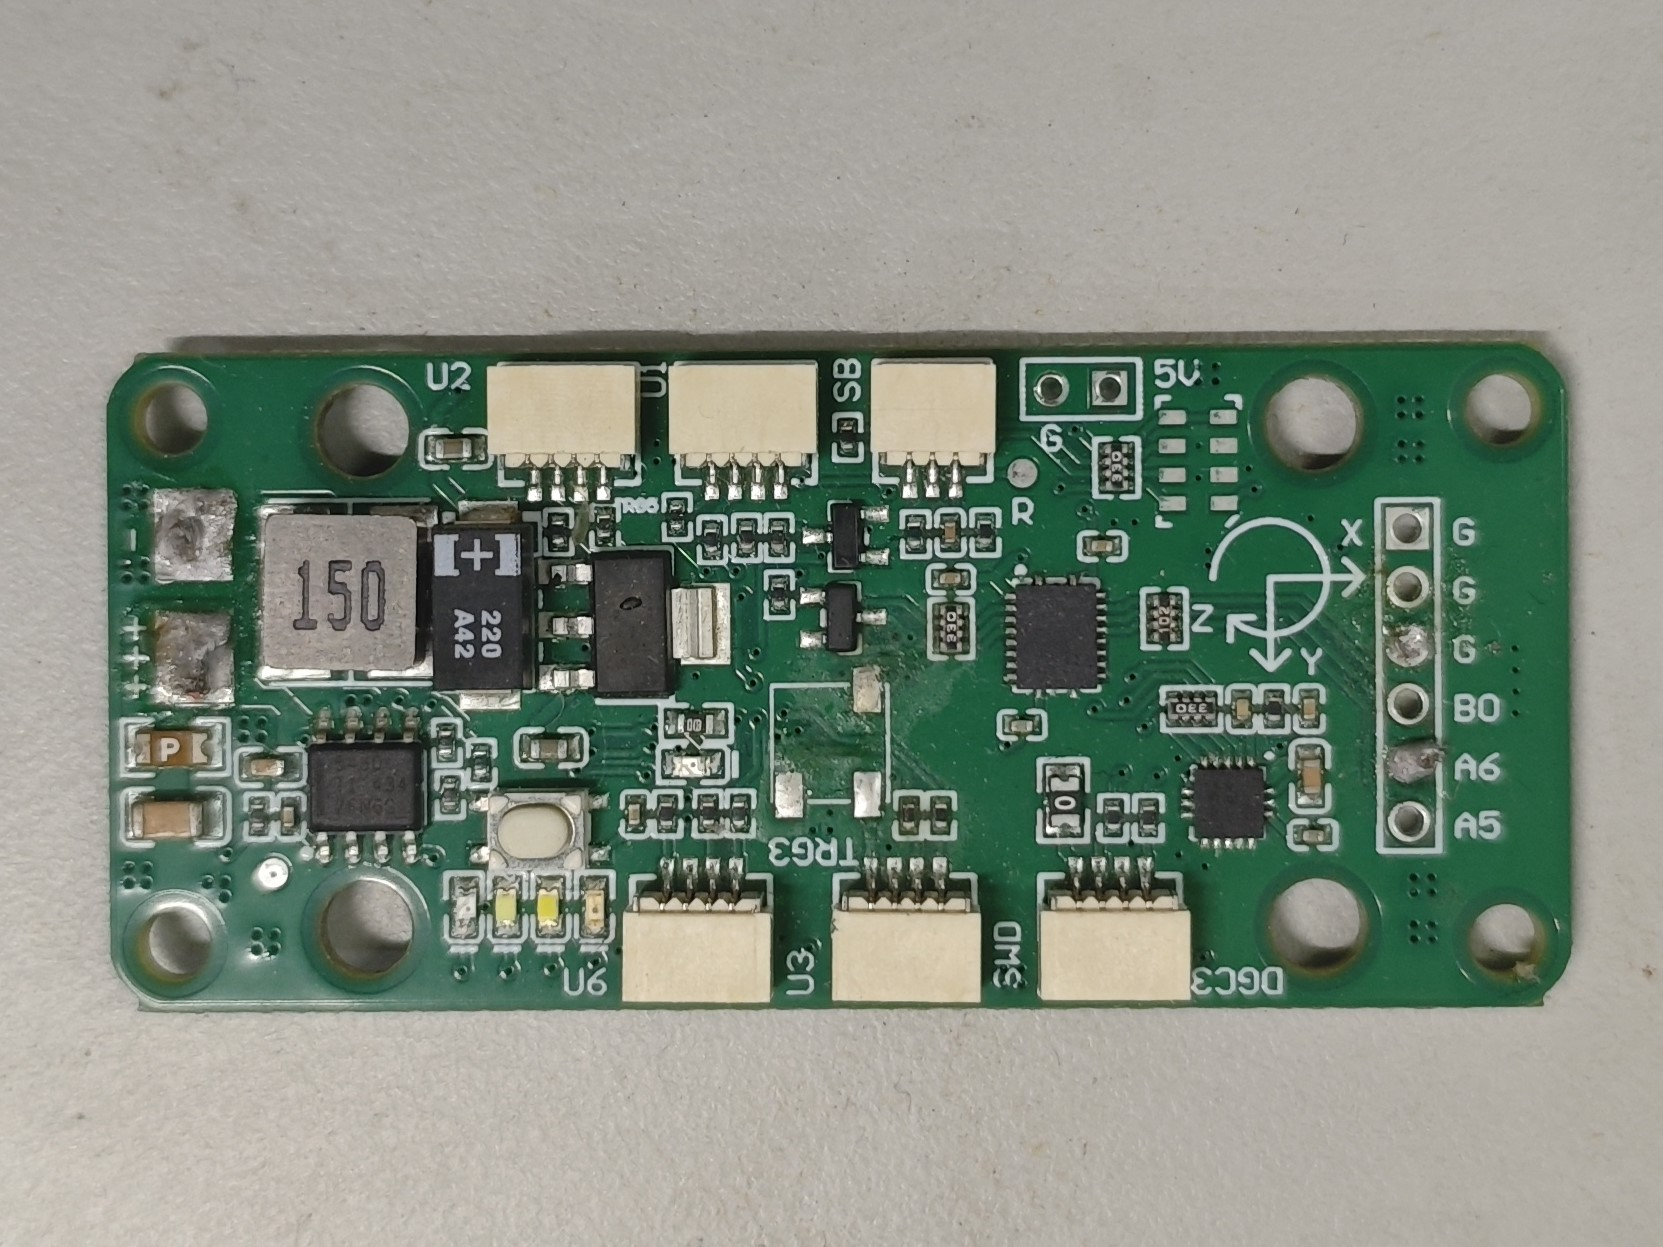
\includegraphics[height=0.18\textheight]{figure/chapter1/main_board.jpg}
            \caption{飞行控制板}
        \end{minipage}
        \hfill  % 产生弹性水平间距
        \begin{minipage}[b]{0.45\textwidth}
            \centering
            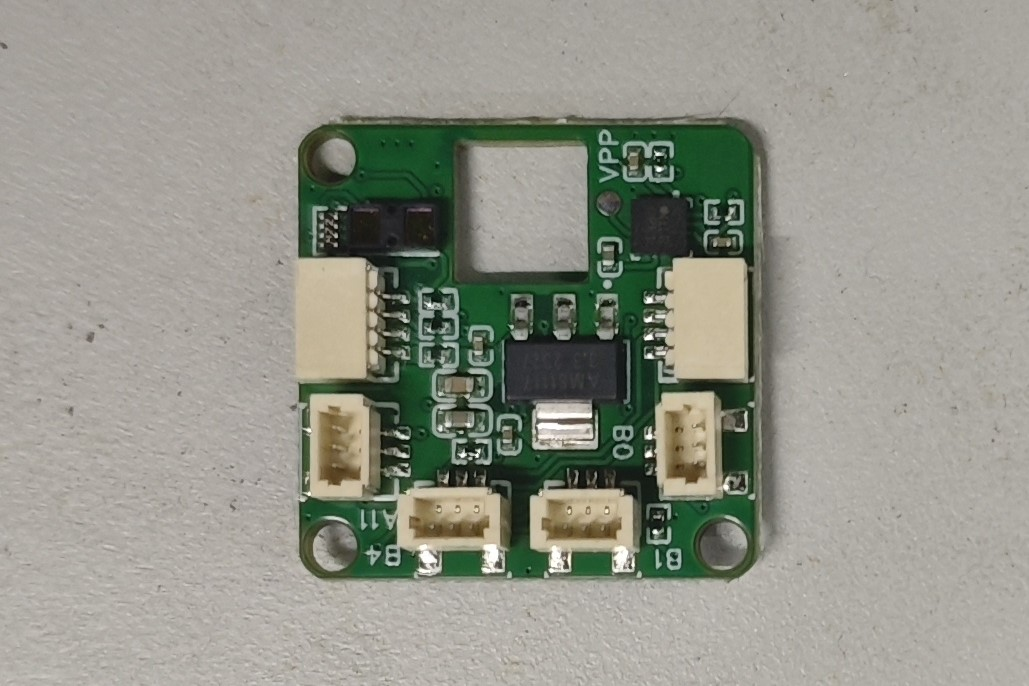
\includegraphics[height=0.18\textheight]{figure/chapter1/slave_board.jpg}
            \caption{舵机驱动板}
        \end{minipage}
    \end{figure}
  \end{itemize}

为明确机载各模块之间的供配电关系与通信链路，本文给出了无人机的电气系统拓扑结构，如图\ref{fig:hardware}所示。该图定义各个电子模块之间的电气连接与信号传输逻辑。
\begin{figure}
    \centering
    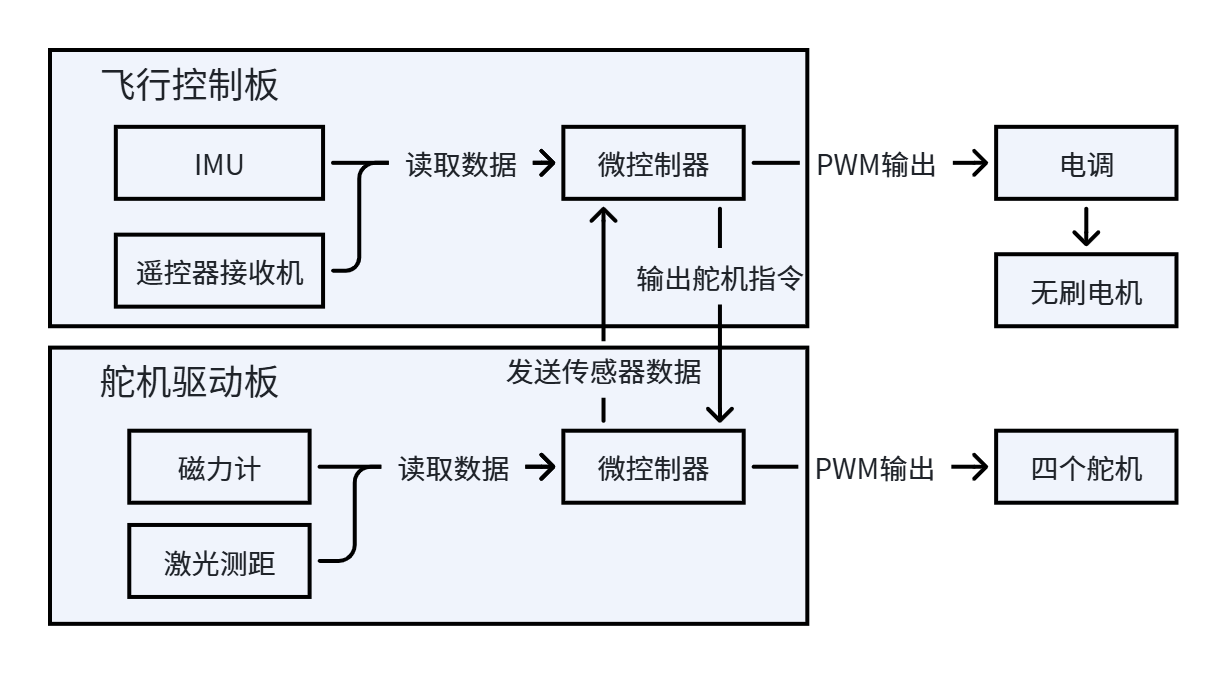
\includegraphics[scale=0.25]{figure/chapter2/hardware_topo.png}
    \caption{\label{fig:hardware}电气系统拓扑结构}
\end{figure}

\subsection{程序设计}
程序设计指的是基于C++语言设计的部署在微控制器上的嵌入式程序设计。为了对多个任务进行调度管理，该程序部署了FreeRTOS实时操作系统。程序主要负责内容如下：遥控器控制指令获取，传感器数据读取，传感器数据预处理，无人机位姿估计，闭环控制器算法处理，输出执行器指令等。具体程序设计如图\ref{fig:software_figure}所示。
\begin{figure}
    \centering
    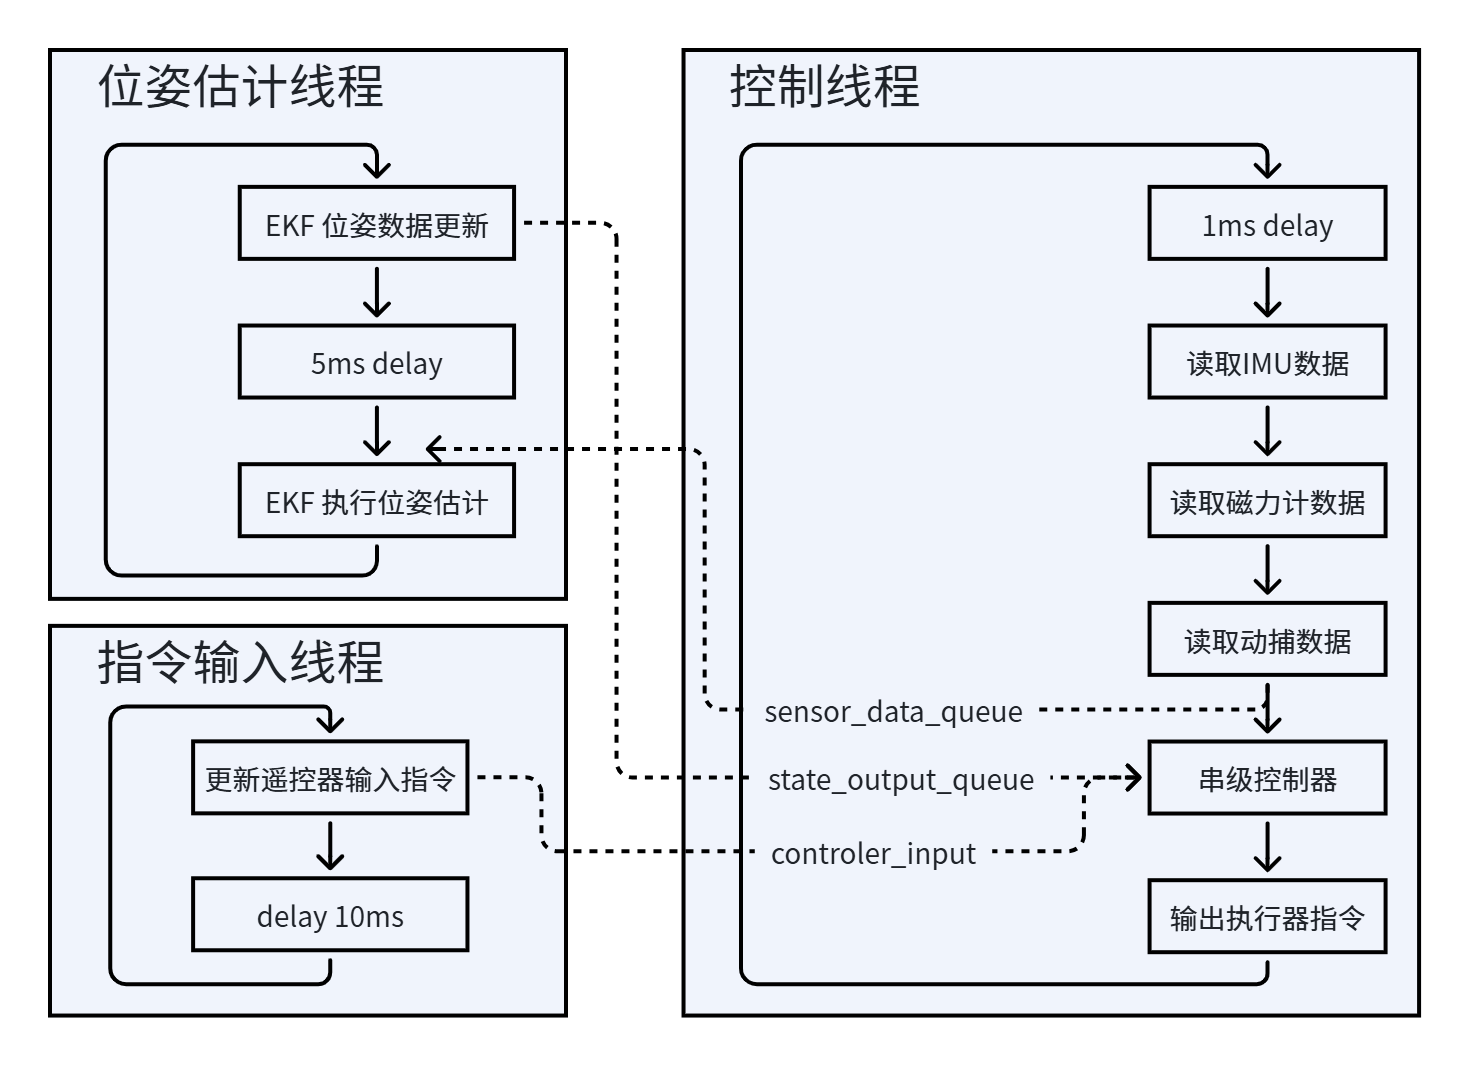
\includegraphics[scale=0.25]{figure/chapter2/software.png}
    \caption{\label{fig:software_figure}程序设计框图}
\end{figure}

\section{坐标系的定义}
坐标系定义是任何飞行器动力学建模与控制系统设计的逻辑起点，其严谨性直接决定了后续数学推导的准确性与结论的可靠性，是后续的模型分析、控制器设计与实验验证理论基础。

\subsection{地面坐标系}
地面坐标系是右手系，满足右手定则。取无人机的起飞点作为地面坐标系的原点\( O_e \)，定义坐标轴\( O_eX_e \)过原点\( O_e \)向地理北向，坐标轴\( O_eY_e \)过原点\( O_e \)向地理东向，由右手定则，坐标轴\( O_eZ_e \) 竖直向下。根据定义可知，该地面坐标系\( O_e - X_e Y_e Z_e \)和地面相对静止，因此，地面坐标系为惯性系。地面坐标系文中也称为地面系。

\subsection{机体坐标系}
机体坐标系也是右手系，同样满足右手定则。取无人机的质心为机体坐标系的原点\( O_b \)，定义坐标轴\( O_bX_b \)过原点\( O_b \)指向无人机的正前方，定义坐标轴\( O_bY_b \)过原点\( O_b \)指向无人机的正右方，由右手定则，坐标轴\( O_bZ_b \) 过原点\( O_b \)指向无人机的正下方。类似的，机体坐标系\( O_b - X_b Y_b Z_b \)和无人机相对静止，机体坐标系为非惯性系。机体坐标系文中也称为机体系。

\begin{figure}
    \centering
    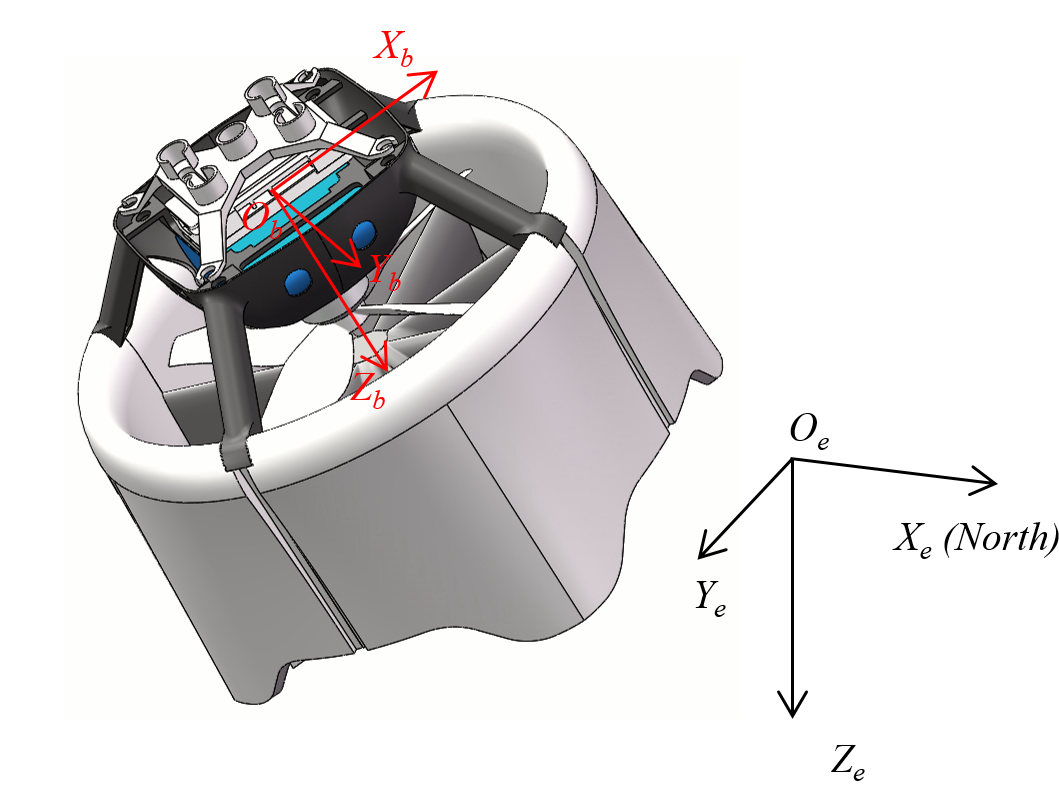
\includegraphics[scale=0.25]{figure/chapter2/coordinary.png}
    \caption{\label{fig:cordinate}地面坐标系和机体坐标系}
\end{figure}

地面坐标系和机体坐标系的关系如图\ref{fig:cordinate}所示。值得注意的是，在三维空间中，同一个矢量，在两个坐标系下的投影是不一样的。为了防止表述上出现歧义，此处定义，三维空间中的矢量在地面坐标系下的投影记为$(·)^e$，在机体坐标系下的投影记为$(·)^b$。

\subsection{坐标系之间的旋转关系}
坐标系之间的旋转关系是进行姿态控制、导航和传感器融合的基础。常用的表示方法主要有四种：欧拉角、旋转矩阵、四元数和轴角法。在现有的飞控程序中，最常用的是欧拉角和四元数。欧拉角是较为直观的表示方式，但是其存在万向锁的问题\cite{quan2018}，当俯仰角为±90°时，会出现自由度退化的问题。由于本文设计的无人机控制的俯仰角不会超过±45°，因此，不需要考虑万向锁所带来的问题。

（1）欧拉角

欧拉角是描述刚体在三维空间中旋转关系的一种常用方法，它通过三次绕指定坐标轴的旋转，将地面坐标系变换到机体坐标系。本文使用的欧拉角是“ZYX欧拉角”，即旋转顺序为：首先绕地面坐标系的 $O_eZ_e$ 轴旋转角度 $\psi$（即偏航角），然后绕新坐标系的 $O_e 'Y_e '$ 轴旋转角度 $\theta$（即俯仰角，最后绕最新坐标系的 $O_e ''X_e ''$ 轴旋转角度 $\varphi$（即滚转角。这种旋转方式也称为内旋，即每次旋转绕当前坐标系的轴进行。
规定$(\psi, \theta, \varphi)$的角度范围为：
\begin{equation}
\psi \in (-\pi,\ \pi], \quad \theta \in \left[-\frac{\pi}{2},\ \frac{\pi}{2}\right], \quad \varphi \in (-\pi,\ \pi].
\end{equation}
\begin{figure}
    \centering
    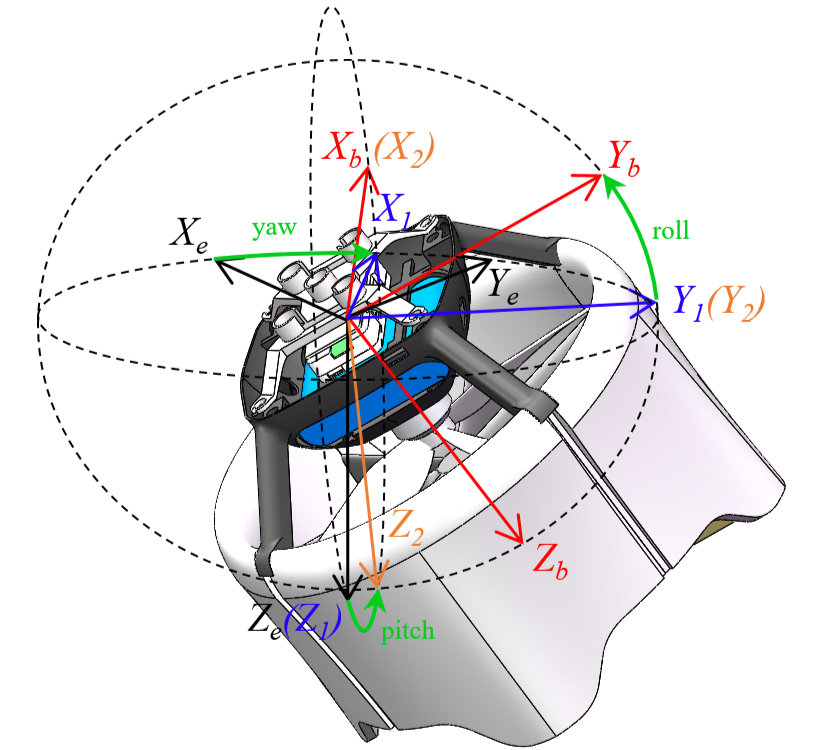
\includegraphics[scale=0.25]{figure/chapter2/eular_angle.png}
    \caption{\label{fig:eular_angle}“ZYX欧拉角”的定义}
\end{figure}

（2）旋转矩阵

定义从机体坐标系到地面坐标系的旋转矩阵 $\boldsymbol{R}_{b}^{e}$，使得对三维空间中的任意矢量$\boldsymbol{v}$ 在机体坐标系中的投影$\boldsymbol{v}^b$ 以及其在地面坐标系中的投影 $\boldsymbol{v}^b$ 满足：
\begin{equation}
\boldsymbol{v}^b = \boldsymbol{R}_{b}^{e} \, \boldsymbol{v}^b.
\end{equation}
根据旋转矩阵的特性，从地面坐标系到机体坐标系的旋转矩阵$\boldsymbol{R}_{e}^{b} = \boldsymbol{R}_{b}^{eT}$ ，且满足：
\begin{equation}
\boldsymbol{v}^b = \boldsymbol{R}_{e}^{b} \, \boldsymbol{v}^b.
\end{equation}
按照上述顺序，旋转矩阵可通过依次左乘每次旋转对应的基本旋转矩阵得到。绕X、Y、Z轴旋转的基本旋转矩阵的定义分别如下：
\begin{equation}
\boldsymbol{R}_x(\varphi) = \begin{bmatrix}
1 & 0 & 0 \\
0 & \cos\varphi & -\sin\varphi \\
0 & \sin\varphi & \cos\varphi
\end{bmatrix},
\boldsymbol{R}_y(\theta) = \begin{bmatrix}
\cos\theta & 0 & \sin\theta \\
0 & 1 & 0 \\
-\sin\theta & 0 & \cos\theta
\end{bmatrix},
\boldsymbol{R}_z(\psi) = \begin{bmatrix}
\cos\psi & -\sin\psi & 0 \\
\sin\psi & \cos\psi & 0 \\
0 & 0 & 1
\end{bmatrix}.
\label{eq:single_eular_R}
\end{equation}

对于ZYX内旋顺序，旋转矩阵 $\boldsymbol{R}_{e}^{b}$ 的计算过程为：

a. 第一次旋转绕地面系 $O_eZ_e$ 轴旋转 $\psi$，得到坐标系 $\{1\}$，有 $\boldsymbol{R}_{e}^{1} = \boldsymbol{R}_z(\psi)$。

b. 第二次旋转绕坐标系 $\{1\}$ 的 $O_e'Y_e'$ 轴旋转 $\theta$，得到坐标系 $\{2\}$。由于旋转在当前坐标系中进行，且当前坐标系的基仍为标准正交基，该旋转在坐标系 $\{1\}$ 中的表示即为 $\boldsymbol{R}_y(\theta)$。因此从世界到坐标系 $\{2\}$ 的旋转矩阵为 $\boldsymbol{R}_{e}^{2} = \boldsymbol{R}_y(\theta) \boldsymbol{R}_z(\psi)$。

c. 第三次旋转绕坐标系 $\{2\}$ 的 $O_e''X_e''$ 轴旋转 $\varphi$，类似地得到从世界到物体坐标系的旋转矩阵：
\begin{equation}
\boldsymbol{R}_{e}^{b} = \boldsymbol{R}_x(\varphi) \boldsymbol{R}_y(\theta) \boldsymbol{R}_z(\psi).
\end{equation}
展开后得从地面坐标系到机体坐标系的旋转矩阵$\boldsymbol{R}_{e}^{b}$：
\begin{equation}
\boldsymbol{R}_{e}^{b} = 
\begin{bmatrix}
\cos\theta\cos\psi & \cos\theta\sin\psi & -\sin\theta \\
\sin\varphi\sin\theta\cos\psi - \cos\varphi\sin\psi & \sin\varphi\sin\theta\sin\psi + \cos\varphi\cos\psi & \sin\varphi\cos\theta \\
\cos\varphi\sin\theta\cos\psi + \sin\varphi\sin\psi & \cos\varphi\sin\theta\sin\psi - \sin\varphi\cos\psi & \cos\varphi\cos\theta
\end{bmatrix}.
\end{equation}

\section{运动学模型}
运动学建模是指在不考虑引起运动的力（如重力、惯性力、摩擦力等）的情况下，使用数学工具对物体或机构的运动属性进行描述、分析和计算的过程。本小节将针对涵道式无人机的机身进行运动学分析，用数学语言建立其位置姿态与时间之间的关系。

记无人机在地面系下的位置矢量为$\boldsymbol{p}$，无人机在地面系下的速度矢量为$\boldsymbol{v}$，记无人机的欧拉角为$\boldsymbol{\eta}=[\varphi \quad \theta \quad \psi]^T$，记无人机的角速度矢量为$\boldsymbol{\omega}$，那么$\boldsymbol{\omega}$在机体系下的投影为$\boldsymbol{\omega}^b = [p \quad q \quad r]^T$。

由速度和位置之间的关系，可得:
\begin{equation}
    \dot{\boldsymbol{p}}^e = \boldsymbol{v}^b = \boldsymbol{R}_b^e \boldsymbol{v}^b.
    \label{eq:d_pos}
\end{equation}

而无人机的角速度和与其欧拉角的关系可参考Ducard等人\cite{Ducard2009Flight}的推导结果，此处直接引述其结论:

\begin{equation}
\boldsymbol{\omega}^b = \dot{\psi} \boldsymbol{R}_\varphi \boldsymbol{R}_\theta \boldsymbol{e}_3 + \dot{\theta} \boldsymbol{R}_\varphi \boldsymbol{e}_2 + \dot{\varphi} \boldsymbol{e}_1,
\label{eq:eular_rate}
\end{equation}
其中，
\begin{equation}
\boldsymbol{e}_1 = 
\begin{bmatrix}
1 \\
0 \\
0
\end{bmatrix}, \quad \boldsymbol{e}_2 = 
\begin{bmatrix}
0 \\
1 \\
0
\end{bmatrix}, \quad \boldsymbol{e}_3 = 
\begin{bmatrix}
0 \\
0 \\
1
\end{bmatrix}.
\label{eq:unit_vector}
\end{equation}
由式\eqref{eq:single_eular_R}，\eqref{eq:eular_rate}，\eqref{eq:unit_vector}，可得：
\begin{equation}
\dot{\boldsymbol{\eta}} = 
\begin{bmatrix}
1 & \sin\varphi\tan\theta & \cos\varphi\tan\theta \\
0 & \cos\varphi & -\sin\varphi \\
0 & \sin\varphi & \cos\varphi
\end{bmatrix}
\boldsymbol{\omega}^b,
\end{equation}
为了简化表述，令矩阵$\boldsymbol{Q}$为：
\begin{equation}
\boldsymbol{Q} = 
\begin{bmatrix}
1 & \sin\varphi\tan\theta & \cos\varphi\tan\theta \\[6pt]
0 & \cos\varphi & -\sin\varphi \\[6pt]
0 & \dfrac{\sin\varphi}{\cos\theta} & \dfrac{\cos\varphi}{\cos\theta}
\end{bmatrix}.
\end{equation}
最终，能够得到无人机的角速度和姿态角的变化率之间的关系为：
\begin{equation}
    \dot{\boldsymbol{\eta}} = \boldsymbol{Q}\boldsymbol{\omega}^b.
    \label{eq:d_eular}
\end{equation}

\section{动力学模型}
动力学建模是指在考虑引起运动的根本原因——力与力矩的前提下，运用物理学基本定律建立数学模型。在动力学建模领域，牛顿-欧拉方法是一种广泛应用于多体系统动力学建模的递推算法，它基于经典力学中的牛顿第二定律和欧拉方程，通过正向和反向递推，系统地建立机器人等机构各连杆之间的运动学关系。和大多数无人机领域的学术研究一样，本文假设涵道式无人机的各个零件认为是质量均匀分布的刚体模型。

由前文对机体结构的介绍可知，涵道式无人机可以看作六个相互独立的刚体，分别是无人机的机身、螺旋桨以及四个控制舵面。四个控制舵面和机体通过转动副连接，涵道风扇和机体也通过转动副连接。由于单个控制舵面的质量仅为3.2g，控制舵面的活动范围较小，为避免动力学模型过于复杂，本文作出必要的简化，认为控制舵面是能够产生气动力而质量为零的刚体，并将控制舵面的质量计入机身质量。

无人机的位置动力学可由牛顿第二定律推导出。记无人机受到的除重力之外的合外力为$\boldsymbol{F}$，无人机质量为$m$，当地重力加速度大小为$g$，无人机的加速度为$\boldsymbol{a}$，由牛顿第二定律可以得到，加速度在地面坐标系下的投影$\boldsymbol{a}^e$为：
\begin{equation}
    \boldsymbol{a}^e = \dot{\boldsymbol{v}}^e = g\boldsymbol{e}_{3} + m^{-1} \boldsymbol{F}^e,
    \label{eq:a_e}
\end{equation}

为方便后续对气动力和气动力矩的研究，本文选用$\boldsymbol{v}^b$作为系统状态量之一，下面推导其动态 $\dot{\boldsymbol{v}}^b$。根据矢量在旋转坐标系中的导数定理，惯性系下的绝对导数与旋转系下的相对导数之间存在如下关系：
\begin{equation}
    \dot{\boldsymbol{v}}^e = \boldsymbol{R}_b^e(\dot{\boldsymbol{v}}^b + \boldsymbol{\omega}^{b} \times \boldsymbol{v}^b).
    \label{eq:transport}
\end{equation}
将式 \eqref{eq:transport} 代入式 \eqref{eq:a_e} 的左端 $\dot{\boldsymbol{v}}^e$，得到：
\begin{equation}
    \boldsymbol{R}_b^e(\dot{\boldsymbol{v}}^b + \boldsymbol{\omega}^{b} \times \boldsymbol{v}^b) = g\boldsymbol{e}_{3} + m^{-1} \boldsymbol{F}^e,
\end{equation}
移项整理得到完全在机体坐标系下表达的平动动力学方程：
\begin{equation}
    \dot{\boldsymbol{v}}^b = g\boldsymbol{R}_e^b\boldsymbol{e}_3 + m^{-1} \boldsymbol{F}^b - \boldsymbol{\omega}^b \times \boldsymbol{v}^b
    \label{eq:d_vel}
\end{equation}

无人机的姿态动力学可由欧拉方程推导出。记无人机受到的合外力矩为$\boldsymbol{M}$，无人机的角动量为$\boldsymbol{L}$，无人机在机体系下的转动惯量矩阵为$\boldsymbol{J}$。
显然，机体系下的转动惯量矩阵$\boldsymbol{J}$是一个常矩阵，且由该无人机结构\ref{fig:body}可以看出，其质量分布关于平面$X_b O_b Z_b$和平面$Y_b O_b Z_b$对称分布，机体坐标系的三个轴均为刚体的惯性主轴，因此，矩阵$\boldsymbol{J}$为对角阵\cite{quan2018}。记$J_x$、$J_y$和$J_z$分别为机体对三轴的主转动惯量，得：
\begin{equation}
    \boldsymbol{J} = 
    \begin{bmatrix}
        J_x & 0 & 0 \\
        0 & J_y & 0 \\
        0 & 0 & J_z
    \end{bmatrix}.
\end{equation}
由欧拉方程，无人机受到的合外力矩在机体坐标系下的投影$\boldsymbol{M}^b$可直接给出：
\begin{equation}
    \boldsymbol{M}^b = \boldsymbol{J}\cdot\dot{\boldsymbol{\omega}^b}+\boldsymbol{\omega}^b\times(\boldsymbol{J}\cdot\boldsymbol{\omega}^b),
\end{equation}
经整理，可得：
\begin{equation}
    \dot{\boldsymbol{\omega}^b} = \boldsymbol{J}^{-1}(\boldsymbol{M}^b - \boldsymbol{\omega}^b\times(\boldsymbol{J}\cdot\boldsymbol{\omega}^b)).
    \label{eq:d_omega}
\end{equation}

至此，无人机的基本运动学和动力学模型可以通过\eqref{eq:d_pos}、\eqref{eq:d_eular}、\eqref{eq:d_vel}、\eqref{eq:d_omega}给出，整理可得：
\begin{equation}
    \begin{cases} 
        \dot{\boldsymbol{p}}^e &= \boldsymbol{R}_b^n \boldsymbol{v}^b \\ 
        \dot{\boldsymbol{v}}^b &= g\boldsymbol{R}_e^b\boldsymbol{e}_3 + m^{-1} \boldsymbol{F}^b - \boldsymbol{\omega}^b \times \boldsymbol{v}^b  \\ 
        \dot{\boldsymbol{\eta}} &= \boldsymbol{Q}\boldsymbol{\omega}^b \\ 
        \dot{\boldsymbol{\omega}^b} &= \boldsymbol{J}^{-1}(\boldsymbol{M}^b - \boldsymbol{\omega}^b\times(\boldsymbol{J}\cdot\boldsymbol{\omega}^b)) 
    \end{cases} .
    \label{eq:base_dynamic}
\end{equation}

值得注意的是，上文的动力学模型中，存在两个未知量$\boldsymbol{F}$和$\boldsymbol{M}$，即无人机受到的除重力以外的合外力和合外力矩。这部分作用力和作用力矩是涵道式无人机的受力分析中最复杂的，也是涵道式无人机所独有的。接下来将展开分析这些力和力矩，以完善整个动力学模型。

\section{涵道式无人机受力分析}
由于涵道式无人机独特的机体结构，其飞行状态下的气动特性相比于多旋翼无人机更为复杂。涵道式无人机在飞行过程中所受到作用，主要包括机身、螺旋桨、控制舵面以及反扭矩襟翼带来的力和力矩。接下来，将根据现有主流理论，对机体受到的各个力和力矩进行逐一分解。

\subsection{涵道风扇动力学}
涵道风扇是指外层由涵道壁包裹的经特殊设计的螺旋桨。在涵道风扇的稳定工作状态下，空气从上方涵道口被吸入，在涵道和涵道风扇的共同作用下，被加速加压，沿涵道轴向从下方涵道口被排出。这个过程由于存在涵道壁对气流的约束和压缩作用，使得涵道风扇相比于孤立旋翼有更高的气动效率。

稳定工作状态下涵道风扇产生的力和力矩，与多种因素存在复杂耦合关系，包括螺旋桨转速、桨盘面积、涵道无人机的迎角、气流速度、无人机飞行速度等。对此，目前数值法分析是学术界的主流研究方法\cite{cheng2021, han2022}。Ohanian等人经过大量试验并通过数值法深入研究后，使用轴向的拉力和垂直于轴向的侧向力的模型来解释涵道风扇产生的总作用力和作用力矩\cite{2012Nondimensional}。在给出其结论之前，需要先定义几个重要的物理量。

\begin{figure}
    \centering
    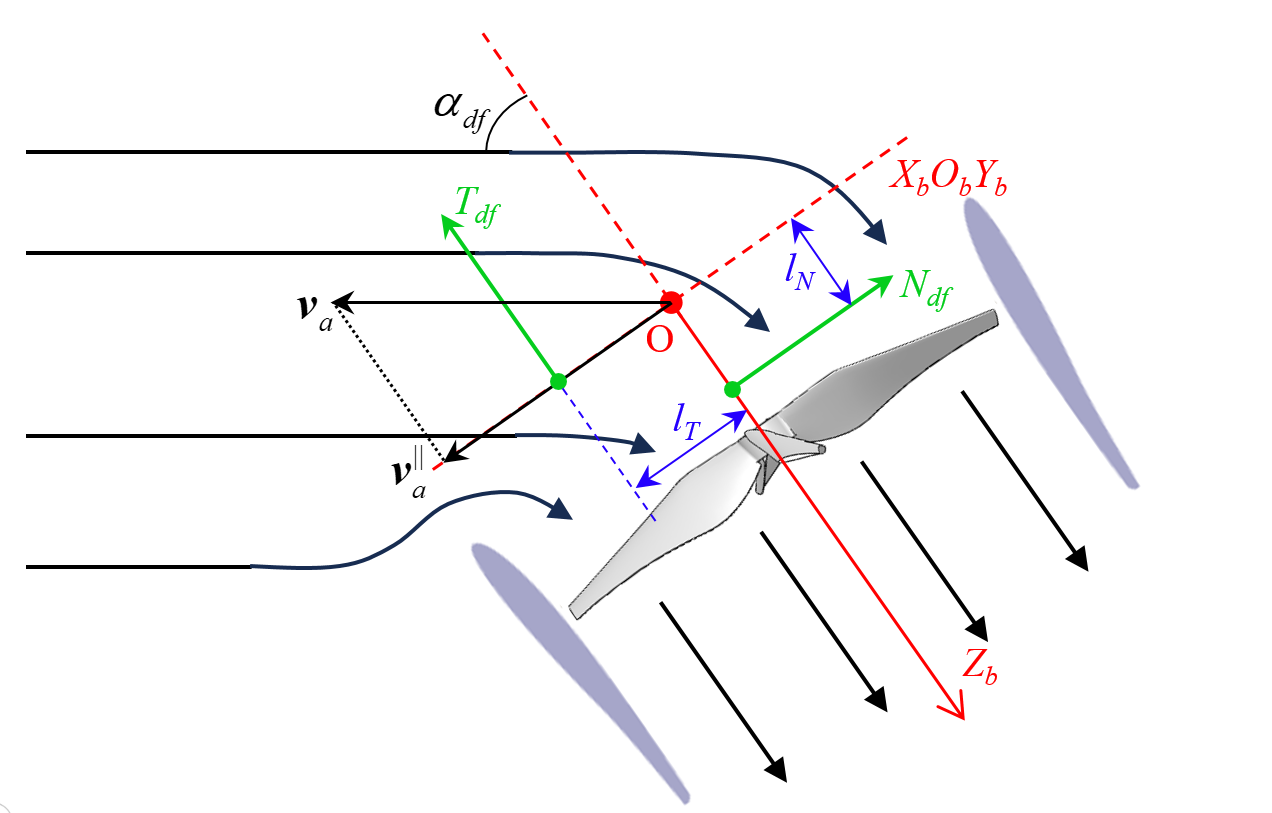
\includegraphics[scale=0.25]{figure/chapter2/ductedfan_force.png}
    \caption{\label{fig:ductedfan_force}涵道风扇气动力分析}
\end{figure}

定义$\Omega$为螺旋桨的角速度大小，$R$为螺旋桨的半径。

定义$\boldsymbol{v}_a$为空速，即机体相对于周围气流的速度，$V_a$为其大小，$\boldsymbol{v}_a^b = [u_r \quad v_r \quad w_r]^T$为其在机体系下的投影。

定义$\boldsymbol{v}_a^{||}$为空速$\boldsymbol{v}_a$在机体系平面$X_bO_bY_b$上的投影，显然，$\boldsymbol{v}_a^{||}$在机体系下的投影为$[u_r \quad v_r \quad 0]^T$。

定义$\alpha_{df}$为涵道迎风角，即空速$\boldsymbol{v}_a$的方向和机体系坐标轴$O_bZ_b$负方向的夹角。

定义$J$为涵道风扇前进比：
\begin{equation}
    J = \frac{\pi V_a}{R \Omega}.
    \label{eq:J}
\end{equation}

图\ref{fig:ductedfan_force}展示了上述多个物理量的几何关系。


(1)涵道风扇的气动力

根据Ohanian等人的理论，拉力$T_{df}$和侧向力$N_{df}$可由下面式子给出\cite{2012Nondimensional}：
\begin{equation}
    \begin{cases}
        T_{df} = \frac{1}{2}\rho \pi C_T R^4 \Omega^2 \\
        N_{df} = \frac{1}{2}\rho \pi C_N R^4 \Omega^2 
    \end{cases}.
    \label{eq:thrust}
\end{equation}
其中，$C_T$和$C_N$都是无量纲系数，分别是涵道风扇的拉力系数和侧向力系数，且它们满足下面式子\cite{2012Nondimensional}：
\begin{equation}
    \begin{cases}
        C_T = C_{T0} + J (C_{T_{J0}} + C_{T_J} \cos\alpha_{df}) \\
        C_N =  J C_{N_J} \sin\alpha_{df}
    \end{cases}.
    \label{eq:thrust_k}
\end{equation}
其中，$C_{T0}$为涵道无人机在悬停状态下的拉力系数，$C_{T_{J0}}$和$C_{T_J}$是拉力随迎风角变化的调整系数，$C_{N_J}$是侧向力随迎风角变化的调整系数。

结合式\eqref{eq:J}，式\eqref{eq:thrust}和式\eqref{eq:thrust_k}可得侧向力$N_{df}$为：
\begin{equation}
    N_{df} = \frac{1}{2}\rho \pi^2 R^3 C_{N_J} V_a \sin\alpha_{df} \Omega.
\end{equation}

已知风扇拉力的方向是指向机体系坐标轴$O_bZ_b$的负方向，那么结合式\eqref{eq:thrust}和式\eqref{eq:thrust_k}，风扇拉力矢量$\boldsymbol{T}_{df}^b$在机体系下的投影可写为：
\begin{equation}
    \boldsymbol{T}_{df}^b = -\frac{1}{2}\rho \pi R^4 \Omega^2 (C_{T0} + J (C_{T_{J0}} + C_{T_J} \cos\alpha_{df})) \cdot \boldsymbol{e}_3.
    \label{eq:T_df}
\end{equation}

已知$N_{df}$的方向与$\boldsymbol{v}_a^{||}$方向相反，注意到，$V_a \sin\alpha_{df}$即为$\boldsymbol{v}_a^{||}$的模，那么侧向力矢量$\boldsymbol{N}_{df}^b$在机体系下的投影可写为：
\begin{equation}
    \boldsymbol{N}_{df}^b = -\frac{1}{2}\rho \pi^2 R^3 C_{N_J} \Omega \cdot \boldsymbol{v}_a^{||} = 
    \begin{bmatrix}
        -\frac{1}{2}\rho \pi^2 R^3 C_{N_J} \Omega u_r \\
        -\frac{1}{2}\rho \pi^2 R^3 C_{N_J} \Omega v_r \\
        0
    \end{bmatrix}.
    \label{eq:N_df}
\end{equation}

涵道风扇受到的总气动力在机体系下的投影$\boldsymbol{F}_{df}^b$即为这两个力的矢量和：
\begin{equation}
    \boldsymbol{F}_{df}^b = \boldsymbol{N}_{df}^b + \boldsymbol{T}_{df}^b =
    \begin{bmatrix}
        -\frac{1}{2}\rho \pi^2 R^3 \Omega C_{N_J} u_r \\
        -\frac{1}{2}\rho \pi^2 R^3 \Omega C_{N_J} v_r \\
        -\frac{1}{2}\rho \pi R^4 \Omega^2 (C_{T0} + J (C_{T_{J0}} + C_{T_J} \cos\alpha_{df}))
    \end{bmatrix}.
\end{equation}

(2)涵道风扇的气动力矩

气动力矩是指涵道风扇的气动力给机体带来的的力矩，从图\ref{fig:ductedfan_force}不难看出，涵道风扇的拉力和侧向力并非经过质心，这些气动力的等效作用点位置的影响因素更为复杂。Ohanian等人所提出的模型是基于侧向力等效作用点不变的假设\cite{2012Nondimensional}，并通过较为简约的解析式描述了涵道风扇气动力矩$M_{df}$：
\begin{equation}
    M_{df} = -l_N N_{df} + l_T T_{df}.
\end{equation}
式中，气动力矩$M_{df}$以使无人机具有抬头趋势的方向为正，$X_J$和$X_{\alpha}$均为无量纲的常系数，$l_N$和$l_T$分别是侧向力和拉力对机体重心的力臂，其关系如图\ref{fig:ductedfan_force}所示。根据该理论，侧向力的作用点固定且高度大致位于涵道入口平面，可认为侧向力力臂$l_N$为已知常量，拉力力臂$l_T$满足如下关系：
\begin{equation}
    l_T = X_J J R \sin(X_\alpha \alpha_{df}).
\end{equation}
将式\eqref{eq:J}代入可得：
\begin{equation}
    l_T = X_J \pi V_a \Omega ^{-1} \sin(X_\alpha \alpha_{df}).
    \label{eq:l_T}
\end{equation}

由图\ref{fig:ductedfan_force}可知，拉力的力臂平行于$\boldsymbol{v}_a^{||}$，那么根据几何关系拉力力臂和侧向力力臂在机体系下的投影$\boldsymbol{L}_T^b$和$\boldsymbol{L}_N^b$可分别写为：
\begin{equation}
    \boldsymbol{L}_T^b = 
    \begin{bmatrix}
        l_T \cdot \dfrac{u_r}{V_a \sin\alpha} \\[8pt]
        l_T \cdot \dfrac{v_r}{V_a \sin\alpha} \\[8pt]
        0 \\[8pt]
    \end{bmatrix} = 
    \begin{bmatrix}
        \dfrac{X_J \pi \sin(X_\alpha \alpha_{df}) u_r}{\Omega \sin\alpha} \\[8pt]
        \dfrac{X_J \pi \sin(X_\alpha \alpha_{df}) v_r}{\Omega \sin\alpha} \\[8pt]
        0 \\[8pt]
    \end{bmatrix},
    \boldsymbol{L}_N^b = 
    \begin{bmatrix}
        0 \\[8pt]
        0 \\[8pt]
        -l_N \\[8pt]
    \end{bmatrix},
\end{equation}
已知力和力臂，即可求出涵道风扇的气动力矩在机体系下的投影$\boldsymbol{M}_{df}^b$：
\begin{equation}
    \begin{aligned}
        \boldsymbol{M}_{df}^b = &\boldsymbol{L}_T^b \times \boldsymbol{T}_{df}^b + \boldsymbol{L}_N^b \times \boldsymbol{N}_{df}^b \\
        =
        &\begin{bmatrix}
            -\dfrac{1}{2}\rho \pi R^4 \Omega^2 (C_{T0} + J (C_{T_{J0}} + C_{T_J} \cos\alpha_{df})) \cdot \dfrac{X_J \pi \sin(X_\alpha \alpha_{df}) u_r}{\Omega \sin\alpha} \\[8pt]
            \dfrac{1}{2}\rho \pi R^4 \Omega^2 (C_{T0} + J (C_{T_{J0}} + C_{T_J} \cos\alpha_{df})) \cdot \dfrac{X_J \pi \sin(X_\alpha \alpha_{df}) u_r}{\Omega \sin\alpha} \\[8pt]
            0 \\[8pt]
        \end{bmatrix} \\
        &+ \begin{bmatrix}
            - \dfrac{1}{2}\rho \pi^2 R^3 \Omega C_{N_J} v_r \cdot l_N \\[8pt]
            \dfrac{1}{2}\rho \pi^2 R^3 \Omega C_{N_J} u_r \cdot l_N \\[8pt]
            0 \\[8pt]
        \end{bmatrix}.
    \end{aligned}
\end{equation}

此外，涵道风扇在高速旋转过程中，会受到与旋转方向相反的力矩，该力矩会通过电机最终传递到机体上，称为涵道风扇反扭距。定义涵道风扇反扭距为$M_{fan}$，该扭矩大小可以由下式给出：
\begin{equation}
    M_{fan} = \frac{1}{2}\rho \pi C_Q R^5 \Omega^2.
\end{equation}

由于本文设计的涵道式无人机的螺旋桨旋转方向指向机体系坐标轴$O_bZ_b$轴正方向，因此该反扭矩指向$Z_b$轴负方向，有：
\begin{equation}
    \boldsymbol{M}_{fan}^b = - M_{fan} \cdot \boldsymbol{e}_3 = - \frac{1}{2}\rho \pi C_Q R^5 \Omega^2 \cdot \boldsymbol{e}_3.
    \label{eq:M_fan}
\end{equation}

(3)涵道风扇的陀螺力矩

陀螺力矩是指若对高速旋转的转子施加一个力矩，使其自转轴发生倾斜，则物体会产生一个垂直于施加力矩方向且垂直于自转轴方向的力矩。本文研究的样机内部的涵道风扇转速较大，在实践过程中发现，其陀螺力矩效应尤为明显。根据其陀螺力矩的定义，陀螺力矩在机体系下的投影$\boldsymbol{M}_{gyro}^b$满足如下关系：
\begin{equation}
    \boldsymbol{M}_{gyro}^b = J_{fan} (\Omega \cdot \boldsymbol{e}_3 \times \boldsymbol{\omega}^b) = 
    \begin{bmatrix}
        -J_{fan} \Omega q \\
        J_{fan} \Omega p \\
        0
    \end{bmatrix}
    \label{eq:M_gyro}
\end{equation}
式中，$J_{fan}$为涵道风扇对转轴的转动惯量。

\subsection{反扭距襟翼动力学}
对于单螺旋桨的涵道式无人机，在悬停状态下，螺旋桨产生的反扭距较大。而反扭矩襟翼能够利用涵道风扇吹出的高速流动的气流经过各个翼面产生如图\ref{fig:M_flap}所示的力，在这些力的共同作用下，能够产生襟翼扭矩$\boldsymbol{M}_{flap}$。经过大量的CFD仿真测试，设计出来的反扭距襟翼能够抵消绝大部分的风扇反扭矩$\boldsymbol{M}_{fan}$。
\begin{figure}
    \centering
    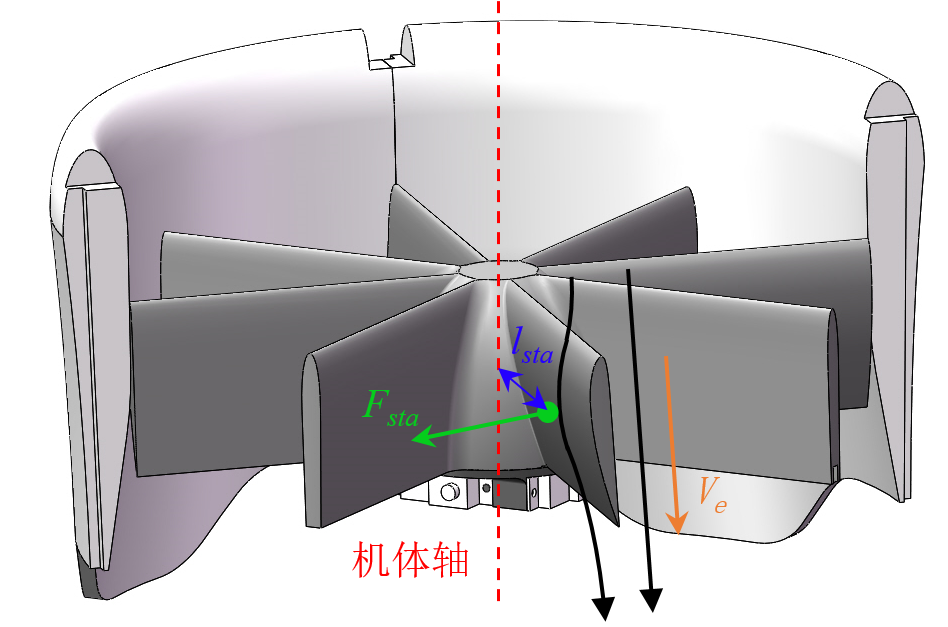
\includegraphics[scale=0.25]{figure/chapter2/anti_torque.png}
    \caption{\label{fig:M_flap}反扭距襟翼作用示意图}
\end{figure}

在给出襟翼扭矩$\boldsymbol{M}_{flap}$与涵道出口风速$V_e$有直接关系，因此，需要先介绍涵道内部的气动特性，以分析出口风速$V_e$。现阶段涵道风扇的气动特性分析的主流理论是基于动量理论与叶素理论展开的。动量理论从整体的角度出发，通过质量、动量和能量守恒定律，建立其推力，功率和气流速度之间的关系。

动量理论的理论前提是，假设气体是定常的不可压缩流体，且流体在任何位置速度不会突变。该理论将涵道风扇看作一个均匀的，厚度无限小的激励盘。如图\ref{fig:flow_status}所示，设气流在无穷远处的速度大小为$V_0$，由于涵道口的抽吸作用，气流流入涵道口的过程中速度逐渐增加并以速度$V_1$接触到涵道风扇的上表面，由于假设认为流体速度不会突变，因此，气流在经过激励盘后，速度仍为$V_1$，而气流压力骤增，紧接着，气流在排出涵道的过程中，气压逐渐降低为外界气压，气流速度进一步增加，最终以速度$V_e$经过涵道出口截面，并被排出。
\begin{figure}
    \centering
    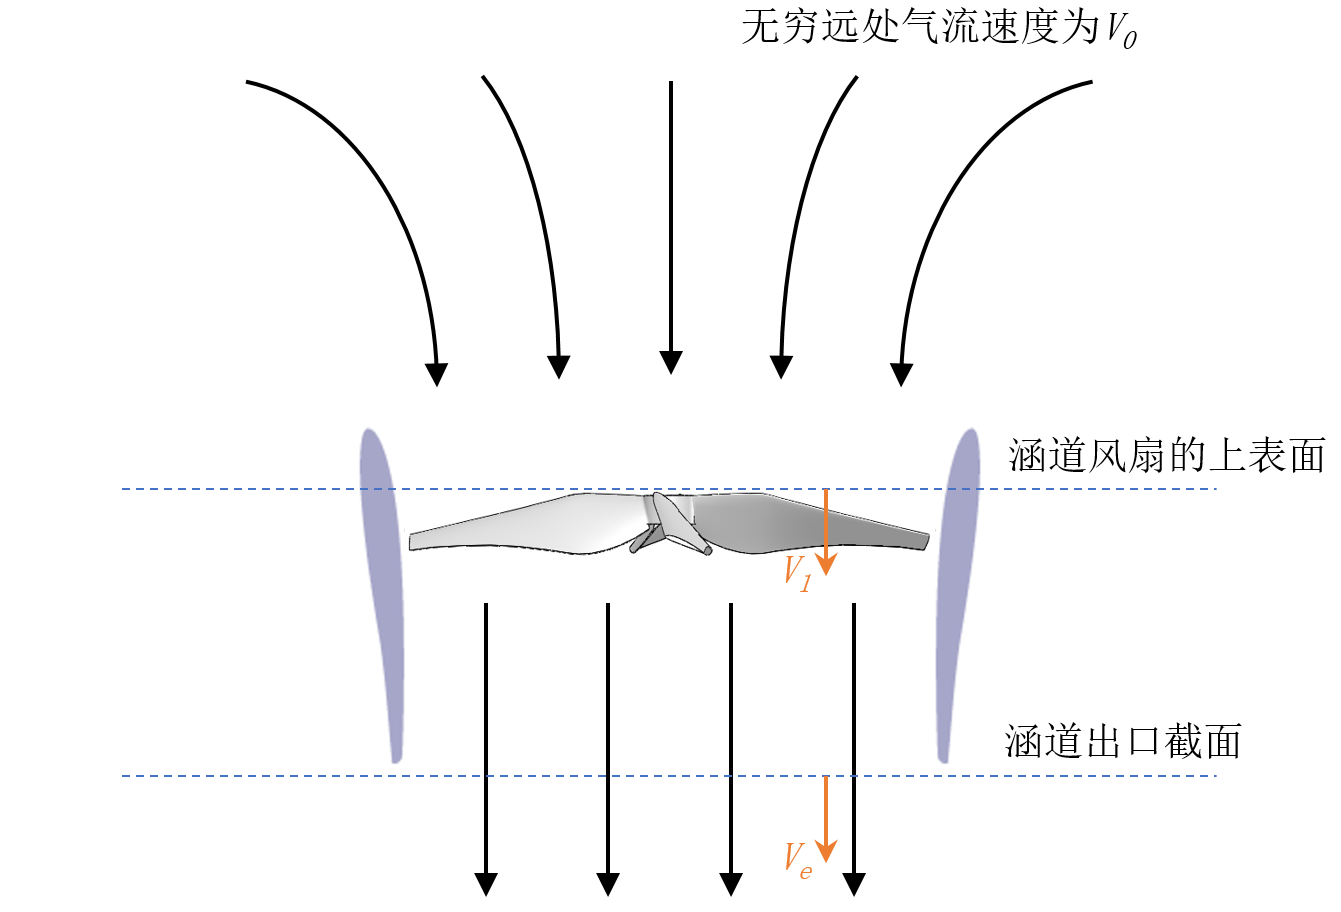
\includegraphics[scale=0.25]{figure/chapter2/ductedfan_flow.png}
    \caption{\label{fig:flow_status}轴流状态的气动分析}
\end{figure}
设单位时间内，从涵道出风口排出的气体质量为$\dot{m}_{air}$，气体密度为$\rho$，根据动量定理可得，涵道风扇对气体的推力等于气流在单位时间内的动量的增加量，即：
\begin{equation}
    T_{df} = \dot{m}_{air} (V_e - V_0) = \rho S V_1 (V_e - V_0),
    \label{eq:dongliang}
\end{equation}
注意到无穷远处的速度为$V_0$的气流和涵道出口处速度为$V_e$的气流，它们的气压一致，均为外界气压，可认为单位时间内，流过出口截面的气体增加的动能即为这部分气体增加的能量。根据能量守恒定律可知，涵道风扇推力的功率等于单位时间内气体动能的变化量：
\begin{equation}
    \frac{1}{2} \dot{m}_{air} V_e^2 - \frac{1}{2} \dot{m}_{air} V_0^2 = T_{df} V_1.
    \label{eq:nengliang}
\end{equation}
此外，设${\sigma}_d$为涵道扩张比，它指的是涵道下方出风口横截面面积$S'$与桨盘面积$S$之比，对于一个结构固定的涵道风扇而言，该扩展比 ${\sigma}_d$ 是常量。那么根据质量守恒定律，有：
\begin{equation}
    \sigma_{d} S V_e = S V_1.
    \label{eq:kuozhangbi}
\end{equation}
联立\ref{eq:dongliang}，\ref{eq:nengliang}和\ref{eq:kuozhangbi}，可得
\begin{equation}
    V_e = \frac{V_0}{2} + \sqrt{(\frac{V_0}{2})^2 + \frac{T_{df}}{{\sigma}_d \rho S}}.
    \label{eq:V_e}
\end{equation}

涵道出口风速$V_e$可近似认为是气流掠过反扭距襟翼的速度，由此便可给出襟翼扭矩的解析表达。襟翼扭矩可以认为各个叶片产生的气动力对机体质心的扭矩的总和。如图\ref{fig:M_flap}，假设单片叶片的面积为$A_{sta}$，叶片的升力系数为$C_{sta}$，单片襟翼产生的升力$F_{sta}$可以表示为：
\begin{equation}
    F_{sta} = \frac{1}{2} \rho A_{sta} C_{sta} V_e^2.
\end{equation}
记叶片数量为$n_{sta}$，单个叶片受到的气动力的压心到机体轴的距离为$l_{sta}$襟翼扭矩$M_{sta}$可以表示为：
\begin{equation}
    M_{sta} = n_{sta} l_{sta} F_{sta} = \frac{n_{sta}}{2} \rho A_{sta} C_{sta} l_{sta} V_e^2.
\end{equation}

襟翼扭矩的方向为机体系坐标轴$O_bZ_b$的正方向，恰与风扇反扭距方向相反，则该扭矩在机体系下的投影$\boldsymbol{M}_{sta}^b$为：
\begin{equation}
    \boldsymbol{M}_{sta}^b = n_{sta} l_{sta} F_{sta} = \frac{n_{sta}}{2} \rho A_{sta} C_{sta} l_{sta} V_e^2 \cdot \boldsymbol{e}_3.
    \label{eq:M_sta}
\end{equation}

\subsection{控制舵面动力学}
\label{subsec:cv_dynamics}
涵道无人机的控制力矩主要来源与控制舵面，利用涵道风扇出风口高速喷射的气流，控制舵面通过调整其角度，来产生合适的升力。由于控制舵面距离无人机质心较远，在正常飞行状态下，能够产生效果较为可观的控制力矩。

如图\ref{fig:ctrl_surface}所示，本文所研究的无人机具有四个控制舵面，每个控制舵面由一对平行翼面构成。定义四个舵面旋转的正方向均为沿转轴方向，从靠近机体轴一侧指向远离机体轴一侧。并且，定义旋转正方向与$O_bX_b$轴同向的舵面为1号舵，反向的舵面为3号舵；定义旋转正方向与$O_bY_b$轴同向的为2号舵，反向的为4号舵。，定义控制舵面的偏转角度向量为$\boldsymbol{\delta} = [\delta_1 \quad \delta_2 \quad \delta_3 \quad \delta_4]^T$，分别对应1，2，3，4号控制舵面。
\begin{figure}
    \centering
    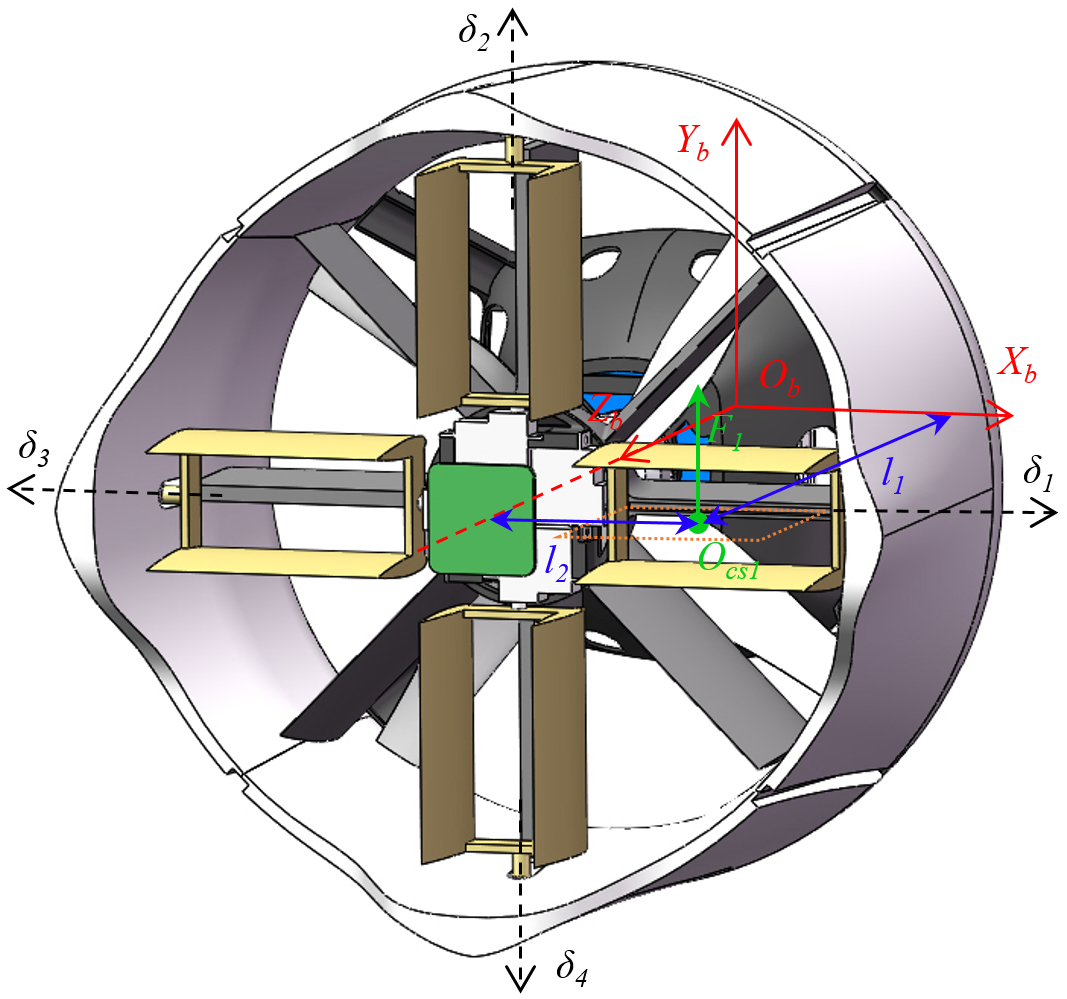
\includegraphics[scale = 0.25]{figure/chapter2/control_surface.png}
    \caption{\label{fig:ctrl_surface}控制舵面示意图}
\end{figure}

针对单个控制舵面，可以认为一对平行翼面的气动压力的压心位于两片翼面的轴对称平面上，如图橙色点虚线平面\ref{fig:ctrl_surface}所示。

在给出控制舵面的气动力之前，有必要先定义几个物理量，如图\ref{fig:ctrl_surface}，设1号控制舵面的气动压力的压心为$O_{cs1}$，$O_{cs1}$到机体系坐标轴$O_bX_b$的距离是$l_1$，$O_{cs1}$到机体系坐标轴$O_bZ_b$的距离是$l_2$，设控制舵面的面积为$A_{cv}$，控制舵面的升力系数为$C_{cv}$。那么根据升力方程，1号舵面单个翼面受到的气动力为：
\begin{equation}
    F_{cv_{1}}' = \frac{1}{2}\rho A_{cv} C_{cv} V_e^2 \delta _1
\end{equation}
单个控制舵面包含一对平行翼面，且四个控制舵面具有对称性，可得各控制舵面受到的气动力：
\begin{equation}
    F_{cv_{i}} = 2 F_{cv_{i}}' = \rho A_{cv} C_{cv} V_e^2 \delta _i, \quad i=1,2,3,4.
\end{equation}

值得注意的是，上述解析式是对控制力的近似，仅当控制舵面偏转角度较小时成立，对此，本文作出限制：
\begin{equation}
    \delta_i \in [-20^\circ, 20^\circ], \quad i=1,2,3,4.
\end{equation}
由于舵面偏转角度较小，可近似认为距离$l_1$，$l_2$均不发生变化。

根据几何关系，并结合式\eqref{eq:F_cv}可得出控制舵面的作用力在机体系下的投影$\boldsymbol{F}_{cv}^b$为：
\begin{equation}
    \boldsymbol{F}_{cv}^b = 
    \begin{bmatrix}
        F_{cv_{4}} - F_{cv_{2}} \\
        F_{cv_{1}} - F_{cv_{3}} \\
        0
    \end{bmatrix} = 
    \begin{bmatrix}
        \rho A_{cv} C_{cv} V_e^2 (\delta _4 - \delta _2) \\
        \rho A_{cv} C_{cv} V_e^2 (\delta _1 - \delta _3) \\
        0
    \end{bmatrix},
    \label{eq:F_cv}
\end{equation}
控制舵面的作用力矩在机体系下的投影$\boldsymbol{M}_{cv}^b$为：
\begin{equation}
    \boldsymbol{M}_{cv}^b = 
    \begin{bmatrix}
        -l_1 (F_{cv_{1}} - F_{cv_{3}}) \\
        l_1 (F_{cv_{4}} - F_{cv_{2}}) \\
        l_2 (F_{cv_{1}} + F_{cv_{2}} + F_{cv_{3}} + F_{cv_{4}})
    \end{bmatrix} = 
    \begin{bmatrix}
        -\rho A_{cv} C_{cv} V_e^2 l_1 (\delta _1 - \delta _3) \\
        \rho A_{cv} C_{cv} V_e^2 l_1 (\delta _4 - \delta _2) \\
        \rho A_{cv} C_{cv} V_e^2 l_2 (\delta _1 + \delta _2 + \delta _3 + \delta _4)
    \end{bmatrix}.
    \label{eq:M_cv}
\end{equation}

\subsection{涵道无人机受力分析总结}
至此，根据现有主流理论，涵道式无人机受到的主要的力和力矩均逐一分析完成。式\eqref{eq:base_dynamic}中的$\boldsymbol{F}^b$和$\boldsymbol{M}^b$可以认为是这些力和力矩的合成，那么在机体系下，有：
\begin{equation}
    \begin{cases}
        \boldsymbol{F}^b = \boldsymbol{F}_{df}^b + \boldsymbol{F}_{cv}^b \\
        \boldsymbol{M}^b = \boldsymbol{M}_{df}^b + \boldsymbol{M}_{fan}^b + \boldsymbol{M}_{gyro}^b + \boldsymbol{M}_{sta}^b + \boldsymbol{M}_{cv}^b
    \end{cases}.
\end{equation}
表\ref{tab:F_and_M}总结了这些力和力矩的符号以及的含义：
\begin{table}
    \caption{\label{tab:F_and_M}涵道式无人机受到的力和力矩}
    \centering{}%
    \begin{tabular}{cc}
    \toprule
    符号 & 含义\tabularnewline
    \midrule
    $\boldsymbol{F}_{df}^b$ & 涵道风扇受到的气动力\tabularnewline
    
    $\boldsymbol{F}_{cv}^b$ & 所有控制舵面受到的气动力的合力\tabularnewline

    $\boldsymbol{M}_{df}^b$ & 涵道风扇受到的气动力对机体的扭矩\tabularnewline

    $\boldsymbol{M}_{fan}^b$ & 涵道风扇受到的反扭距\tabularnewline

    $\boldsymbol{M}_{gyro}^b$ & 螺旋桨因陀螺效应的受到的陀螺力矩\tabularnewline

    $\boldsymbol{M}_{sta}^b$ & 反扭距襟翼受到气动力的对机体的扭矩\tabularnewline

    $\boldsymbol{M}_{cv}^b$ & 所有控制舵面受到的气动力对机体的合扭矩\tabularnewline
    \bottomrule
    \end{tabular}
\end{table}

结合涵道式无人机的运动学模型和动力学模型，可以推导出无人机的完整动态方程。设无人机的状态矢量为：
\begin{equation}
    \boldsymbol{x}_{uav} = 
    \begin{bmatrix}
        \boldsymbol{p}^{e} \\
        \boldsymbol{v}^{b} \\
        \boldsymbol{\eta} \\
        \boldsymbol{\omega}^{b}
    \end{bmatrix},
\end{equation}
且满足：
\begin{equation}
    \boldsymbol{p}^e = 
    \begin{bmatrix}
        p_x^e \\
        p_y^e \\
        p_z^e
    \end{bmatrix},
    \quad
    \boldsymbol{v}^b = 
    \begin{bmatrix}
        v_x^e \\
        v_y^e \\
        v_z^e
    \end{bmatrix}, 
    \quad
    \boldsymbol{\eta} = 
    \begin{bmatrix}
        \phi \\
        \theta \\
        \psi
    \end{bmatrix},
    \quad
    \boldsymbol{\omega^b} = 
    \begin{bmatrix}
        p \\
        q \\
        r
    \end{bmatrix}.
\end{equation}
那么可以给出如下所示的无人机的各个状态量的动态方程。

(1)位置动态方程：
\begin{equation}
    \begin{aligned}
        \dot{p_x^e} =& (\cos\theta\cos\psi) v_x^b + (\sin\varphi\sin\theta\cos\psi - \cos\varphi\sin\psi) v_y^b \\
        &+ 
        (\cos\varphi\sin\theta\cos\psi + \sin\varphi\sin\psi) v_z^b \\
        \dot{p_y^e} =& (\cos\theta\sin\psi) v_x^b + (\sin\varphi\sin\theta\sin\psi + \cos\varphi\cos\psi) v_y^b \\
        &+ 
        (\cos\varphi\sin\theta\sin\psi - \sin\varphi\cos\psi) v_z^b \\
        \dot{p_z^e} =& (-\sin\theta) v_x^b + (\sin\varphi\cos\theta) v_y^b + 
        (\cos\varphi\cos\theta) v_z^b
    \end{aligned}
    \label{eq:p_dynamic}
\end{equation}

(2)速度动态方程：
\begin{equation}
    \begin{aligned}
        \dot{v_x^b} =& -g\sin\theta + m^{-1}(-\frac{1}{2}\rho \pi^2 R^3 \Omega C_{N_J} u_r + \rho A_{cv} C_{cv} V_e^2 (\delta_4 - \delta_2)) \\
        &+ (v_y^e r - v_z^e q)\\
        \dot{v_y^b} =& g\sin\phi\cos\theta + m^{-1}(-\frac{1}{2}\rho \pi^2 R^3 \Omega C_{N_J} v_r + \rho A_{cv} C_{cv} V_e^2 (\delta_1 - \delta_3)) \\
        &+ (v_z^e p - v_x^e r)\\
        \dot{v_z^b} =& g\cos\phi\cos\theta + m^{-1}(-\frac{1}{2}\rho \pi R^4 \Omega^2 (C_{T0} + J (C_{T_{J0}} + C_{T_J} \cos\alpha_{df}))) \\
        &+ (v_x^e q - v_y^e p)
    \end{aligned}
    \label{eq:v_dynamic}
\end{equation}

(3)姿态动态方程：
\begin{equation}
    \begin{aligned}
        \dot{\varphi} &= p + \sin\varphi \tan\theta \, q + \cos\varphi \tan\theta \, r \\
        \dot{\theta}  &= \cos\varphi \, q - \sin\varphi \, r \\
        \dot{\psi}    &= \frac{\sin\varphi}{\cos\theta} \, q + \frac{\cos\varphi}{\cos\theta} \, r
    \end{aligned}
    \label{eq:eta_dynamic}
\end{equation}

(4)角速度动态方程：
\begin{equation}
    \label{eq:w_dynamic}
    \begin{aligned}
        \dot{p} = & \frac{1}{J_x} \biggl\{ (J_y - J_z)qr \\[4pt]
        &+ \biggl[ - \frac{1}{2}\rho \pi R^4 \Omega^2 (C_{T0} + J (C_{T_{J0}} + C_{T_J} \cos\alpha_{df})) \cdot \dfrac{X_J \pi \sin(X_\alpha \alpha_{df}) v_r}{\Omega \sin\alpha} \\[4pt]
        & - \frac{1}{2}\rho \pi^2 R^3 \Omega C_{N_J} v_r l_N - J_{{fan}} \Omega q - \rho A_{cv} C_{cv} V_e^2 l_1 (\delta_1 - \delta_3) \biggr] \biggr\} \\[4pt]
        \dot{q} = & \frac{1}{J_y} \biggl\{(J_z - J_x)pr \\[4pt]
        &+ \biggl[  \frac{1}{2}\rho \pi R^4 \Omega^2 (C_{T0} + J (C_{T_{J0}} + C_{T_J} \cos\alpha_{df})) \cdot \dfrac{X_J \pi \sin(X_\alpha \alpha_{df}) u_r}{\Omega \sin\alpha} \\[4pt]
        & + \frac{1}{2}\rho \pi^2 R^3 \Omega C_{N_J} u_r l_N + J_{{fan}} \Omega p + \rho A_{cv} C_{cv} V_e^2 l_1 (\delta_4 - \delta_2) \biggr] \biggr\} \\[4pt]
        \dot{r} = & \frac{1}{J_z} \biggl\{ (J_x - J_y)pq \\[4pt]
        &+\biggl[ - \frac{1}{2}\rho \pi C_Q R^5 \Omega^2  + \rho A_{cv} C_{cv} V_e^2 l_2 (\delta_1 + \delta_2 + \delta_3 + \delta_4) \\[4pt]
        & + \frac{n_{sta}}{2} \rho A_{sta} C_{sta} l_{sta} V_e^2 \biggr] \biggr\}
    \end{aligned}
\end{equation}


\section{实验样机}
\label{sec:sample_uav}
在本文的研究中涉及到模型参数辨识以及基于模型的抗扰控制，其本质上是在利用模型构建一个对现实物理系统的“反向映射”或“逆动力学”，模型的精度直接决定了这一映射的保真度与有效性。因此需要要在开展正式研究前，获取非线性系统的相关参数。经过大量测试、仿真和验证，本文研究的涵道式无人机相关系统参数被整理成表\ref{tab:params}。
\begin{table}
    \caption{\label{tab:params}实验样机非线性系统模型参数}
    \centering{}%
    \begin{tabular}{cccc}
    \toprule
    参数符号 & 数值 & 参数符号 & 数值\tabularnewline

    \midrule 
    $m\mathrm{(kg)}$ & $0.4850$ & $R\mathrm{(m)}$ & $0.089$\tabularnewline

    $J_x,J_y(kg \cdot m^2)$ & $1.632 \times 10^{-3}$ & $J_z\mathrm{(kg \cdot m^2)}$ & $8.567 \times 10^{-4}$\tabularnewline

    $l_1\mathrm{(m)}$ & $0.09529$ & $l_2\mathrm{(m)}$ & $0.05685$\tabularnewline

    $l_{sta}\mathrm{(m)}$ & $0.03252$ & $n_{sta}$ & $4$\tabularnewline

    $J_{fan}\mathrm{(kg \cdot m^2)}$ & $2.084 \times 10^{-5}$ & $l_N\mathrm{(m)}$ & $0.012$\tabularnewline

    $A_{sta}\mathrm{(m^2)}$ & $2.680 \times 10^{-3}$ & $A_{cv}\mathrm{(m^2)}$ & $2.443 \times 10 ^{-3}$\tabularnewline

    $\rho \mathrm{(kg/m^3)}$ & $1.225$ & $\sigma _d$ & $0.7800$\tabularnewline

    $C_{cv} $ & $1.7266$ & $\sigma _d$ & $0.7800$\tabularnewline
    
    $C_{T0}$ & $ 0.0307$ & $C_{sta}$ & $0.7517$\tabularnewline
    
    $C_{T_{J}}$ & $−0.0691$ & $C_{N_{J}}$ & $0.0959$\tabularnewline
    
    $X_J$ & $0.4679$ & $X_{\alpha}$ & $0.8$\tabularnewline
    
    $C_{Q}$ & $0.0031$\tabularnewline
    \bottomrule
    \end{tabular}
\end{table}

尽管前文通过机理分析建立了涵道式无人机的非线性数学模型，并在理想条件下对其动力学特性进行了推导与部分仿真验证。但必须指出的是，由于涵道无人机在飞行过程中表现出较强的非线性特性，并且与系统的多个状态存在复杂耦合关系，该模型本质上是对真实物理系统的一种理想化抽象与近似描述。在实际工程应用中，由于模型简化、装配误差和机械磨损，理论模型与实物系统之间往往存在一定的偏差。

\section{本章小结}
本章围绕小型涵道式无人机的系统建模展开，旨在建立能够准确描述其运动特性与受力机理的数学模型，为后续的控制器设计和参数辨识提供理论依据。

首先，本章介绍了实验样机的硬件构成，明确了机体结构、动力单元、感知元件与控制执行机构的配置关系。在此基础上，定义了地面坐标系与机体坐标系，并引入ZYX欧拉角描述二者的旋转变换，为姿态解算和运动分析奠定了统一的参考框架。

在运动学层面，基于刚体假设，推导了无人机的位置、速度与姿态角之间的微分关系；在动力学层面，采用牛顿-欧拉法建立了无人机的平动与转动方程，并给出了转动惯量矩阵的表达形式。

针对涵道式无人机特有的气动环境，本章进一步分析了其所受的主要力和力矩，包括涵道风扇产生的拉力与侧向力、反扭矩襟翼的平衡力矩、控制舵面的操纵力以及陀螺效应等。参考现有理论，给出了各气动分量的解析表达，揭示了涵道结构对气流组织和力产生机制的耦合影响，为后续近地面扰动分析与抗扰控制器设计提供了可用的模型基础。从理论层面能够实现对涵道式无人机这一复杂非线性系统的预测以及仿真。

值得注意的是，考虑到理论误差，结构装配误差，机械磨损，模型简化等因素，模型仍存在少量可接受范围内的偏差，这部分需要通过算法的鲁棒性来弥补

本章工作系统梳理了涵道无人机的建模流程，兼顾理论完备性与工程可行性，为后续章节的研究内容奠定了必要的数学与物理基础。
